%!TEX root = main.tex

\section{Regular Expressions a la JavaScript}\label{sec-rwre}
In this section, we introduce the regular expressions which will be used in the string constraints. The semantics of the regular language conforms to the JavaScript language. It should be emphasized that the strings accepted by the regular expresses introduced here are still regular, but the parsing of the string is significantly different from classic regular languages. For this purpose, we utilize prioritized finite-state automata \cite{BM17}, which extend classic finite-state automata with priorities, to capture, among others, the greedy/lazy semantics of Kleene star/plus. 

Throughout the paper, $\Int^+$ denotes the set of positive integers, and  $\nat$ denotes the set of natural numbers. Furthermore, for $n\in \Int^+$, let $[n]:=\{1, \ldots, n\}$. 
%
We use $\Sigma$ to denote a finite set of letters, called \emph{alphabet}. A \emph{string} over $\Sigma$ is a finite sequence of letters from $\Sigma$. We use $\Sigma^*$ to denote the set of strings over $\Sigma$ and $\varepsilon$ to denote the empty string. Moreover, for convenience, we use $\Sigma^\varepsilon$ to denote $\Sigma \cup \{\varepsilon\}$. A string $w'$ is called a \emph{prefix} of $w$ if $w = w'w''$ for some string $w''$. We use $\pref(w)$ to denote the set of prefixes of $w$. For a prefix $w_1$ of $w$, let $w = w_1 w_2$, then we use $w_1^{-1}w$ to denote $w_2$.


%%%%%%%%%%%%%%%%%%%%%%%%%%%%%%%%%%%%%%%%%
%\hide{
%	\tl{this part can be moved to intro?}
%	Regular expressions are a well-known concept in formal language. %and  have the same expressibility as finite state automata. 
%	Many programming languages provide build-in regular expressions %capabilities either built-in 
%	or otherwise via libraries. Programmers widely use regular expressions in software development, especially in the development of web applications. However, it should be emphasized that regular expressions used in programming languages are considerably different from those in formal language theory, mainly on the following aspects: greedy/non-greedy semantics of the quantifiers ($*$ and its variant $+$), non-commutativity of the alternation operator, capturing groups, and backreferences. In the sequel, we take all these aspects into account and define the class of real-world regular expressions considered in this paper. 
%}
%%%%%%%%%%%%%%%%%%%%%%%%%%%%%%%%%%%%%%%%%  

\begin{definition}[Regular expressions, $\regexp$]
	
\begin{multline*}
e \eqdef \emptyset \mid \varepsilon \mid a \mid [e^?] \mid [e^{??}] \mid  (e) \mid %\$n \mid 
[e + e] \mid [e \concat e] \mid \\
[e^*] \mid [e^+] \mid [e^{*?}] \mid  [e^{+?}] \mid [e^{\{m_1,m_2\}}] \mid [e^{\{m_1,m_2\}?}] 
\end{multline*}
%	
where $a \in \Sigma$,  $n \in \Int^+$, $m_1,m_2 \in \Nat$ with $m_1 \le m_2$. 
	%	Since $+$ is associative and commutative, we also write $(e_1 + e_2) + e_3$ as $e_1 + e_2 + e_3$ for brevity.  
\end{definition}
%We abbreviate $[e \concat [e^*]]$ as $[e^+]$ and $[e \concat [e^{*?}]]$ as $[e^{+?}]$. 
%
For $\Gamma = \{a_1, \ldots, a_k\}\subseteq \Sigma$, we write $\Gamma$ for  $[[\cdots [a_1 + a_2] + \cdots] + a_k]$ and thus $[\Gamma^\ast] \equiv [[[\cdots [a_1 + a_2] + \cdots] + a_k]^\ast]$. Similarly for $[\Gamma^{\ast?}]$, $[\Gamma^+]$, and $[\Gamma^{+?}]$. We write $|e|$ for the length of $e$, i.e. the number of symbols occurring in $e$.
%
Note that square brackets $[]$ are used for the operator precedence and the parentheses $()$ are used for \emph{capturing groups}. 
 %
%Parenthesis pairs are indexed according to the occurrence sequence of their left parentheses, and it is required that every back reference $\$ n$ occurs after the $n$-th pair of parentheses. For instance, $[[([[a+b]^*]) \concat c] \concat \$1]$ is in $\regexp$, where $\$1$ refers to the matching of the subexpression $[[a+b]^*]$. Intuitively, it denotes the set of strings of the form $u c u$, where $u$ is a string of $a$ and $b$. 
%

The operator $[e^*]$ is the \emph{greedy} Kleene star, meaning that $e$ should be matched as many times as possible. In contrast, the operator $[e^{*?}]$ is the \emph{lazy} Kleene star, meaning $e$ should be matched  as few times as possible. The Kleene plus operators $[e^+]$ and $[e^{+?}]$ are similar to $[e^*]$ and $[e^{*?}]$ but $e$ should be matched at least once. Moreover, as expected,  $[e^{\{m_1,m_2\}}]$ requires the number of times that $e$ is matched is between $m_1$ and $m_2$ and $[e^{\{m_1,m_2\}?}]$ is the lazy variant. Likewise, the optional operator has greedy and lazy variants $[e^?]$ and $[e^{??}]$, respectively.
 
% 
%We use $\cgexp$ to denote the fragment of $\regexp$ excluding backreferences $\$ n$ (where {\sf reg} represents regular languages), and $\refexp$ to denote the set of regular expressions generated by a concatenation of letters and backreferences, formally %regular expressions 
%defined by $e \eqdef \varepsilon \mid a \mid \$n \mid [e \concat e]$.  
%%\tl{define the semantics here?}

 

\paragraph{Semantics}
We now define the formal semantics of $\regexp$. Traditionally, regular expressions are interpreted as a regular language, i.e., a set of strings, which can be defined inductively in a rather straightforward way. In our case when the regular expression is used in string constraints arisen from analysis of programming language such as JavaScript, %owing to the introduction of greedy/lazy semantics,  
what we need is not only the language denoted by the regular expression, but also the intermediate result when parsing a string against the given regular expression. This is especially the case when the capturing group is involved. As a result, we need a more operational (as opposed traditional denotational) account of the semantics for regular expression. To this end, we harness an extension of finite-state automata with priorities, which \emph{defines} how a string is accepted by the given regular expression. We start with the standard finite-state automaton.  


%\subsection{Semantics of \regexp[\sf CG]}
%In this section, we give one of the many semantics of \regexp[\sf CG], which we will utilize for $\replaceall$.
%For two indexed $\regexp$s $e$ and $e'$, we say $e'$ is a \emph{subexpression} of $e$,
%if one of the following conditions holds: 1) $e'=e$, 2) $e = [e_1 \cdot e_2]$ or $[e_1 + e_2]$, and $e'$ is a subexpression of $e_1$ or $e_2$, 3) $e = [e^?], [e^{??}], [e_1^{\ast}]$, $[e_1^{+}]$, $[e_1^{\ast?}]$, $[e_1^{+?}]$, $e_1^{\{m_1, m_2\}}$, $e_1^{\{m_1, m_2\}?}$ or $(_n e_1)_n$, and $e'$ is a subexpression of $e_1$. We use $S(e)$ to denote the set of all subexpressions of $e$. %\tl{is there a difference between $[e_1\cdot e_2]$ and $e_1 e_2$?}
%
% 
%By a mutual induction on $|w|$ and $|e|$, we can show that $|\cM_{w}(e)|$, the size of $\cM_{w}(e)$, is at most $|w||e|$.  

%\begin{example}\label{exmp-regex-match-tree}
%	Let $w= 0250$ and $e = [[([\Gamma^+])\concat .?] \concat ([\Gamma^*])]$ where $\Gamma = \{0,1,\cdots,9\}$. Note that $e$ is essentially {\tt decimalReg} in the motivating example. Then $\cM_{w}(e) = \{T_1,T_2,T_3, T_4\}$ as illustrated in Figure~\ref{fig-regex-semantics-decimal}(i), (ii), (iii), and (iv), where the match trees rooted at $(0, \Gamma)$, $(2, \Gamma)$, and $(5, \Gamma)$ are omitted. % to avoid tediousness.
%	\begin{figure}[htb]
%		\centering
%		%\rule{\linewidth}{0cm}
%		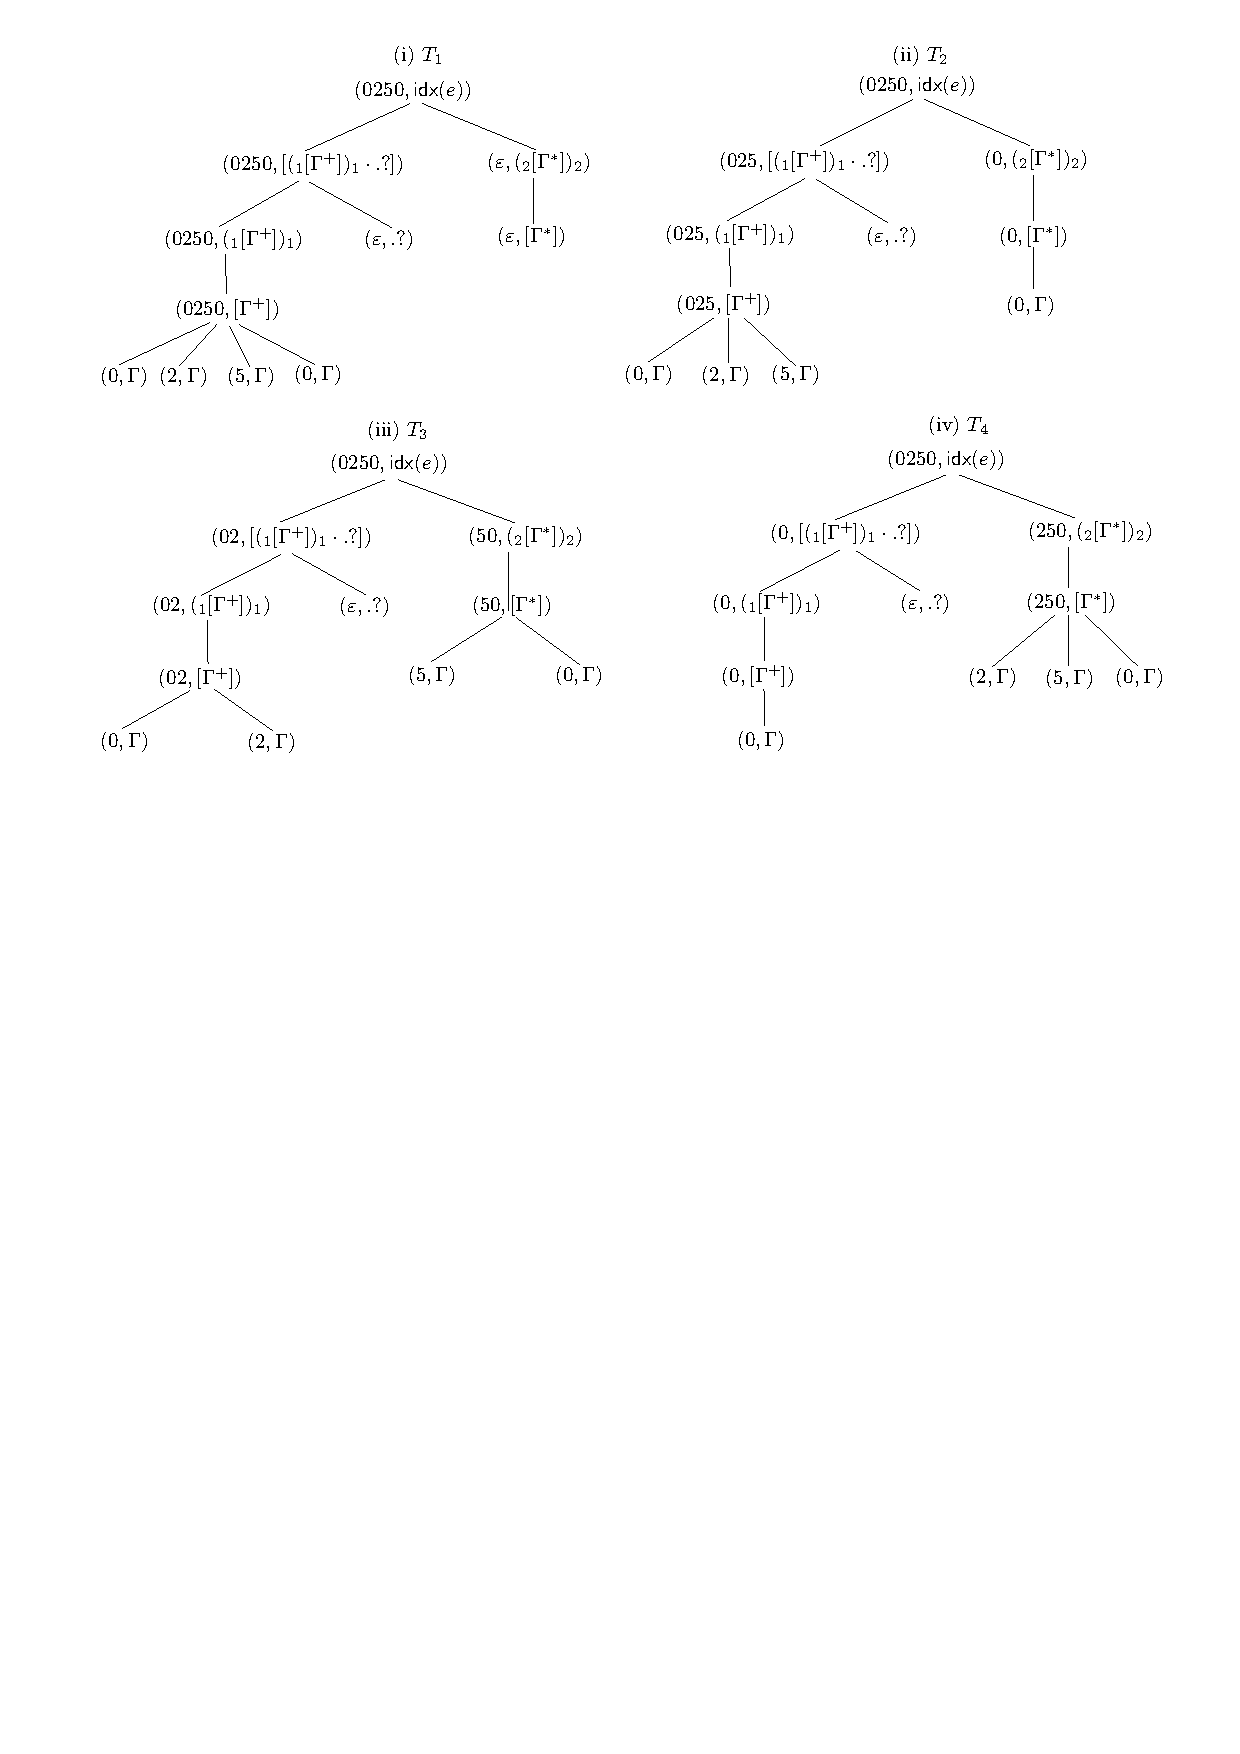
\includegraphics[width=1\textwidth]{regex-semantics-decimal.pdf}
%		\caption{Match trees of $e=[[([\Gamma^+])\concat .?] \concat ([\Gamma^*])]$ to $w= 0250$}
%		\label{fig-regex-semantics-decimal}
%		
%	\end{figure}
%	%\Blindtext
%\end{example}

 
 
%
%\begin{example}\label{exmp-regex-semantics}
%	Let us continue Example~\ref{exmp-regex-match-tree}.  In Fig.~\ref{fig-regex-semantics-decimal}, we have $(T_1)_{(0250, [\Gamma^+])} >_{(w, \idxexp(e))} (T_2)_{(025, [\Gamma^+])}$, since $(0, \Gamma)(2, \Gamma)(5,\Gamma)$ is a proper prefix of $(0, \Gamma)(2, \Gamma)(5,\Gamma)(0, \Gamma)$. Then we deduce that $(T_1)_{(0250, (_1[\Gamma^+])_1)} >_{(w, \idxexp(e))} (T_2)_{(025, (_1[\Gamma^+])_1)}$. Consequently, $(T_1)_{(0250, [(_1[\Gamma^+])_1 \concat .?])} >_{(w, \idxexp(e))} (T_2)_{(025,  [(_1[\Gamma^+])_1 \concat .?])}$ and $T_1 >_{(w, \idxexp(e))} T_2$. Similarly, we have $T_2 >_{(w, \idxexp(e))} T_3$ and $T_3 >_{(w, \idxexp(e))} T_4$. Therefore, $T_1$ is the accepting match of $e$ to $w$, where the first and second capturing group of $e$ are matched to $0250$  and $\varepsilon$ respectively. 
%	%\Blindtext
%\end{example}

%\begin{remark}
%	Our semantics of $\regexp$ follows the 11th Edition of the ECMAScript specification (ES11 for short) \cite{ECMAScript11}, with a focus on the non-commutative union, the greedy/lazy semantics of Kleene star/plus, as well as capturing groups and backreferences.
%	In comparison, POSIX regular expressions require the leftmost and longest match of regular expressions, which we leave as future work.
%\end{remark}


% some examples

%  e = b(a*)a*
%  
%  e' = b(a*?)a*

\begin{definition}[Finite-state Automata] \label{def:nfa}
	A \emph{(nondeterministic) finite-state automaton}
	(\FA{}) over a finite alphabet $\ialphabet$ is a tuple $\Aut =
	(\ialphabet, \controls, q_0, \finals, \transrel)$ where 
	$\controls$ is a finite set of 
	states, $q_0\in \controls$ is
	the initial state, $\finals\subseteq \controls$ is a set of final states, and 
	$\transrel\subseteq \controls \times 
	\ialphabet^\varepsilon \times  \controls$ is the
	transition relation. 
\end{definition}


For an input string $w$, a \emph{run} of $\Aut$ on $w$
%(with $a_0 = \EndLeft$ and $a_{n+1} = \EndRight$)
is a sequence $q_0 a_1 q_1 \ldots a_n q_n$ such that $w = a_1 \cdots a_n$ and $(q_{j-1}, a_{j}, q_{j}) \in
\transrel$ for every $j \in [n]$.
%
The run is said to be \defn{accepting} if $q_n \in \finals$.
A string $w$ is \defn{accepted} by $\Aut$ if there is an accepting run of
$\Aut$ on $w$. 
%In particular, the empty string $\varepsilon$ is accepted by $\Aut$ if $q_0 \in F$. 
The set of strings accepted by $\Aut$, i.e., the language \defn{recognized} by $\Aut$, is denoted by $\Lang(\Aut)$.
%Since we deal with computational complexity in the sequel, we define
The \defn{size} $|\Aut|$ of $\Aut$ is the cardinality of the set $Q$ of states. 

%
For a finite set $Q$, let $\overline{Q} = \bigcup_{n\in \Nat}\{ (q_1, \ldots, q_n) \mid \forall i \in [n], q_i \in Q \wedge \forall i,j \in[n], i \neq j \rightarrow q_i \neq q_j \}$. Intuitively, $\overline{Q}$ is the set of sequences of non-repetitive elements from $Q$. In particular, the empty sequence $\varepsilon \in \overline{Q}$. Note that the length of each sequence from $\overline{Q}$ is bounded by  $| Q |$. For a sequence $P = (q_1, \ldots, q_n) \in \overline{Q}$ and  $q \in Q$, we write $q \in P$ if  $q = q_i$ for some $i \in [n]$. Moreover, for $P_1 = (q_1, \ldots, q_m) \in \overline{Q}$ and $P_2 = (q'_1, \ldots, q'_n) \in \overline{Q}$, we say $P_1 \cap P_2 = \emptyset$ if $\{q_1, \ldots, q_m\} \cap \{q'_1, \ldots, q'_n\} = \emptyset$.

\begin{definition}[Prioritized Finite-state Automata]\label{def-pfa}
	A \emph{prioritized finite-state automaton} (PFA) over a finite alphabet $\Sigma$ is a tuple $\pnfa=(Q, \Sigma, \delta, \tau, q_0, F)$ where $\delta \in Q
	\times \Sigma \rightarrow \overline{Q}$ and $\tau \in Q \rightarrow \overline{Q} \times \overline{Q}$ such that for every $q \in Q$, if $\tau(q) = (P_1; P_2)$, then $P_1 \cap P_2 = \emptyset$. 
	The definition of $Q$, $q_0$ and $F$ is the same as FA.
\end{definition}
For $\tau(q)=(P_1; P_2)$, we will use $\pi_1(\tau(q))$ and $\pi_2(\tau(q))$ to denote $P_1$ and $P_2$ respectively.  With slight abuse of notation, we write $q\in (P_1; P_2)$ for $q\in P_1\cup P_2$. Intuitively, $\tau(q)=(P_1; P_2)$ specifies the $\varepsilon$-transitions at $q$, with the intuition that the $\varepsilon$-transitions to the states in $P_1$ (resp. $P_2$) have higher (resp. lower) priorities than the non-$\varepsilon$-transitions out of $q$.

A \emph{run} of $\pnfa$ on a string $w$ is a sequence $q_0 a'_1 q_1 \ldots a'_m q_m$ such that 
\begin{itemize}
	%\item $q_m \in F$,
	\item for any $i \in [m]$, either $a'_i \in \Sigma$ and $q_i \in \delta (q_{i - 1}, a'_i)$, or $a'_i = \varepsilon$ and $q_i \in \tau(q_{i-1})$, %\pi_1(\tau(q_{i-1}))\cup \pi_2(\tau(q_{i-1}))$,
	\item $w = a'_1 \cdots a'_m$,
	%
	\item for every subsequence $q_i a'_{i+1} q_{i+1} \ldots a'_{j} q_j$ such that  $i < j$ and $a'_{i+1} = \cdots = a'_j = \varepsilon$, it holds that for every $k, l: i \le k < l < j$, $(q_k, q_{k+1}) \neq (q_l, q_{l+1})$.
	%each state $q \in Q$ occurs \emph{at most twice} in the subsequence. 
	(Intuitively, each transition occurs at most once in a sequence of $\varepsilon$-transitions.) 
	%
	%\item moreover, for every suffix $q_i a'_{i+1} q_{i+1} \ldots a'_{m} q_m$ such that $i < m$ and $a'_{i+1} = \cdots = a'_m = \varepsilon$, it holds that $q_i, \dots, q_m$ are mutually distinct.  (Intuitively, each state occurs at most once in a suffix of $\varepsilon$-transitions.) 
\end{itemize}

Note that it is possible that $\delta(q, a) = ()$, that is, there is no $a$-transition out of $q$. 
It is easy to observe that, given a string $w$, the length of a run of $\pnfa$ on $w$ is $O(|w||\cA|)$. 
For any two runs $R = q_0 a_1 q_1 \ldots a_m q_m$ and $R' =  q_0 a'_1 q_1' \ldots a'_n q'_n$ such that $a_1 \ldots a_m = a'_1 \ldots a'_n$, we say that $R$ is of a higher priority over $R'$ if 
\begin{itemize}
	\item either $R'$ is a prefix of $R$ (in this case, the transitions of $R$ after $R'$ are all $\varepsilon$-transitions), 
	%
	\item or there is an index $j$ satisfying one of the following constraints:
	\begin{itemize}
		\item $q_0 a_1 q_1 \ldots q_{j-1} a_j = q_0 a'_1 q'_1 \ldots q'_{j-1} a'_j$, $q_j \neq q'_j$, $a_j \in \Sigma$, and $\delta (q_{j - 1}, a_j) =(\ldots, q_j, \ldots, q_j', \ldots)$,
		%
		\item $q_0 a_1 q_1 \ldots q_{j-1} a_j = q_0 a'_1 q'_1 \ldots q'_{j-1} a'_j$, $q_j \neq q'_j$, $a_j  = \varepsilon$,  and one of the following conditions holds: (i) $\pi_1(\tau(q_{j - 1})) = (\ldots, q_j, \ldots, q_j', \ldots)$, (ii) $\pi_2(\tau(q_{j - 1})) = (\ldots, q_j, \ldots, q_j', \ldots)$, or (iii) $q_j \in \pi_1(\tau(q_{j - 1}))$ and $q'_j \in \pi_2(\tau(q_{j-1}))$, 
		%
		\item $q_0 a_1 q_1 \ldots q_{j-1}  = q_0 a'_1 q'_1 \ldots q'_{j-1} $, $a_j  = \varepsilon$, $a'_j  \in \Sigma$, $q_j \in \pi_1(\tau(q_{j - 1}))$, and $q'_j \in \delta(q_{j-1}, a'_j)$, 
		%
		\item $q_0 a_1 q_1 \ldots q_{j-1}  = q_0 a'_1 q'_1 \ldots q'_{j-1} $, $a_j  \in \Sigma$, $a'_j  = \varepsilon$, $q_j \in \delta(q_{j - 1}, a_j)$, and $q'_j \in \pi_2(\tau(q_{j-1}))$.
	\end{itemize}
\end{itemize}
%From the definition of ``higher priorities" above, we observe that if there is a  run of $\pnfa$ on a string $w$, then there is a unique run of $\pnfa$ on $w$ with the highest priority. 
An \emph{accepting} run of $\pnfa$ on $w$ is a run $R = q_0 a_1 q_1 \ldots a_m q_m$ of $\pnfa$ on $w$ satisfying that 1) $q_m \in F$, 2) $R$ is of the \emph{highest} priority among those runs satisfying $q_m \in F$. 
%(Note that a run $q_0 a_1 q_1 \ldots a_m q_m$ of $\pnfa$ on $w$ with the highest priority may not satisfy $q_m \in F$.) 

The language of $\pnfa$, denoted as $\Lang(\pnfa)$, is the set of strings on which $\pnfa$ has an accepting run.
%
Note that the priorities in PFAs have no impact on whether a string is accepted; they only affect the way that a string is accepted. Therefore, PFAs still define the class of regular languages. 

%\begin{figure}[ht]
%\centering
%\rule{\linewidth}{0cm}
%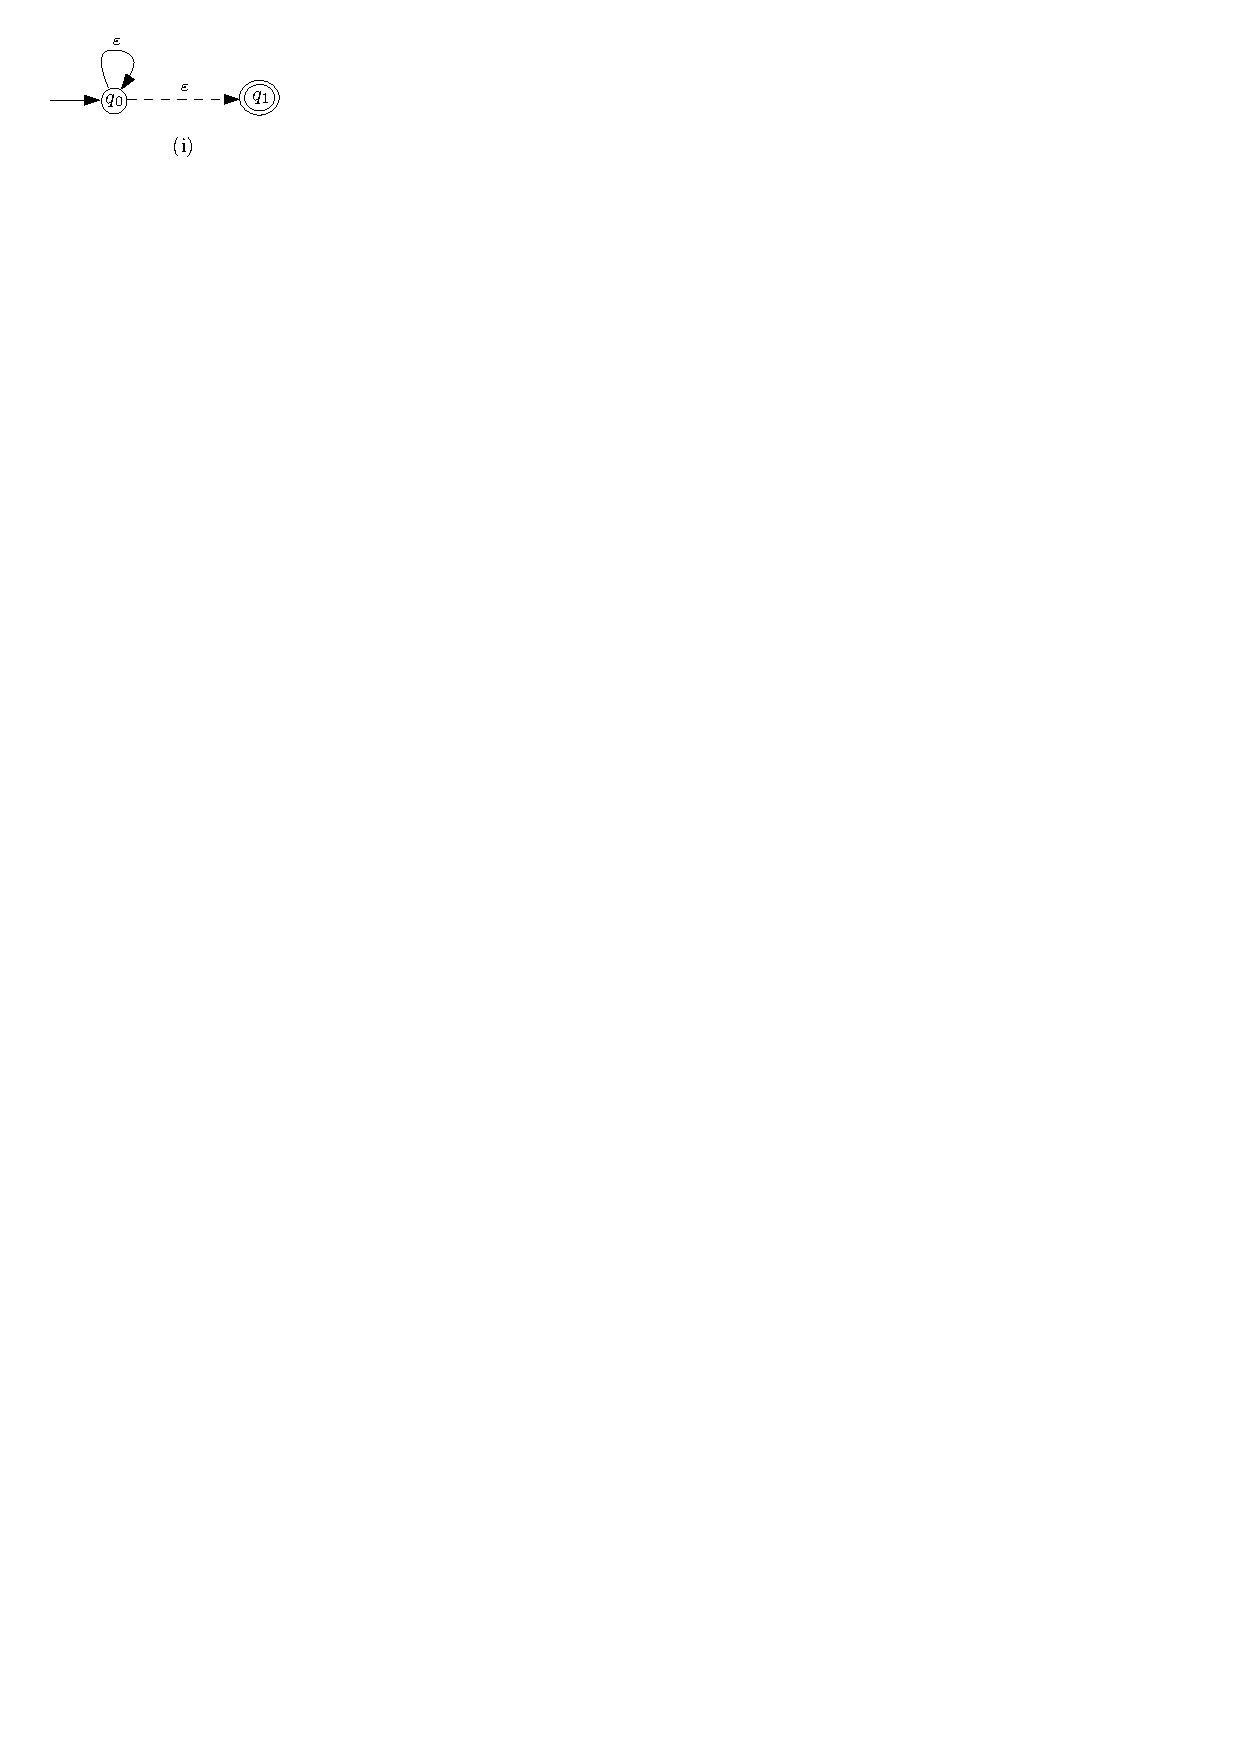
\includegraphics[scale=0.8]{pfa-epsilon-star.pdf}
%\caption{The PFA for $\varepsilon^\ast$}
%\label{fig-pfa-epsilon-star}
%\end{figure}



\begin{example}\label{exmp-pfa}
	The PFA corresponding to the RWRE $e = [[([\Gamma^+])\concat .?] \concat ([\Gamma^*])]$ 
	%in Example~\ref{exmp-regex-match-tree}
	%
	 is illustrated in Fig.~\ref{fig-pfa}, where the dashed (resp. thicker solid) lines represent the $\varepsilon$-transitions of lower (resp. higher) priorities than non-$\varepsilon$ transitions (if there is any), and the doubly circled states are final states. For instance, $\delta(q_1, \ell) = (q_1)$ for every $\ell \in \{0, \dots, 9\}$, $\delta(q_1, .) = ()$, $\tau(q_1) = ((); (q_2))$. Since the $\varepsilon$-transition has lower priority than the $\ell$-transition at the state $q_1$, whenever the currently scanned letter is $\ell \in \{0,\cdots,9\}$ at $q_1$,  the PFA will choose to go to $q_1$ greedily, until there is no more $\ell  \in \{0,\cdots,9\}$. (In this case, it has to choose the $\epsilon$-transition and goes to $q_2$.)
	%
	\begin{figure}[ht]
		
		\centering
		%\rule{\linewidth}{0cm}
		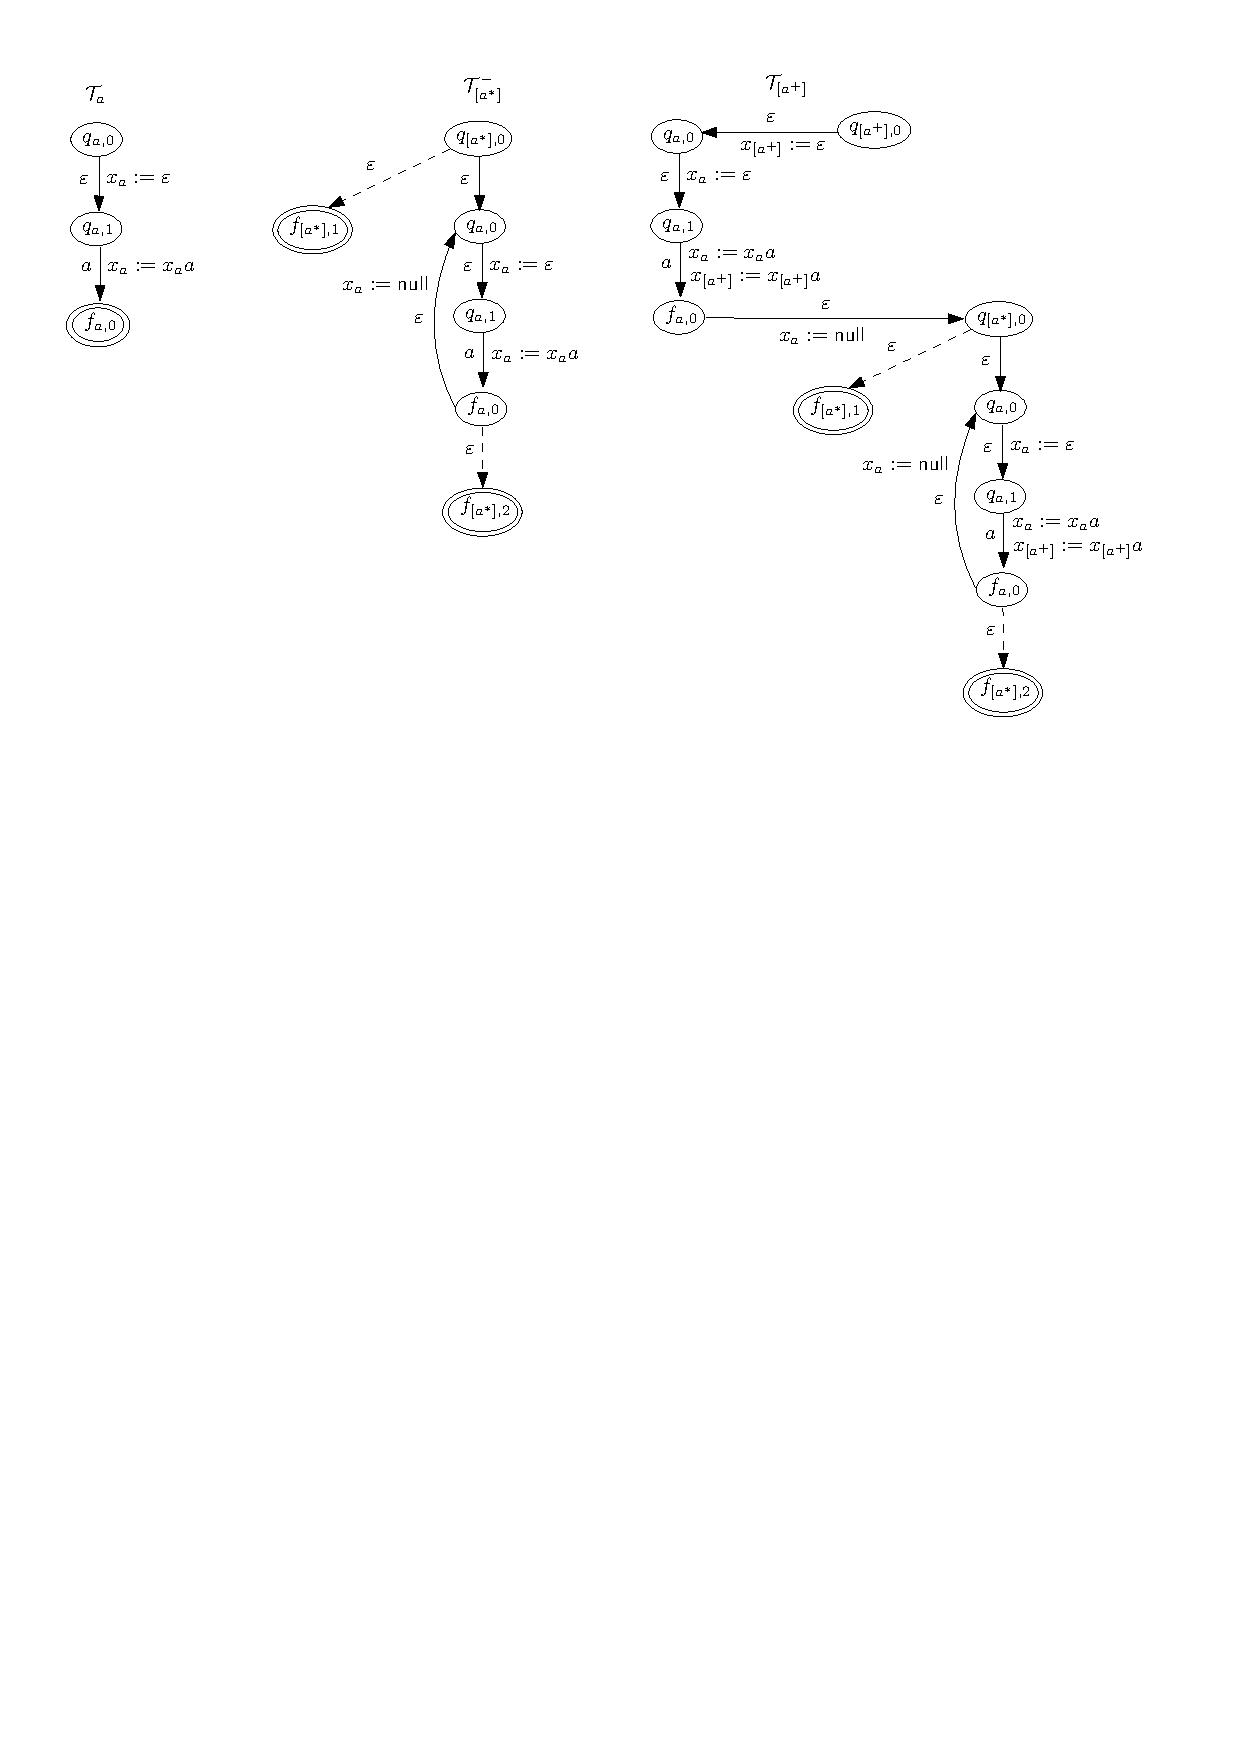
\includegraphics[width=0.9\textwidth]{pfa-new.pdf}
		\caption{The PFA for $e = [[([\Gamma^+])\concat .?] \concat ([\Gamma^*])]$, where $\Gamma = \{0, \cdots, 9\}$}
		\label{fig-pfa}
		
	\end{figure}
\end{example}

%%%%%%%%%%%%%%%%%%%%%%%%%%%%%%%%%%%%%%%%%%%%%%%%%%%%%%%%%%%%%%%%%%%%%%%%%%%%%%%%%%%%%%%%%%%%

%We can adapt the PFA construction in \cite{BDM14}, which in turn is a variant of the standard Thompson construction \cite{Thompson68}, and show the following result. 

%\begin{proposition}\label{prop-rwre-to-pfa}

We associate with each $\cgexp$ $e$ a PFA $\cA_e$ and we define the semantics of $e$ as the language accepted by $\cA_e$. As expected, the construction of PFA is done inductively. 

\paragraph{Case $e =\emptyset$} $\cA_e = (\{q_{\emptyset, 0}\}, \Sigma, \delta, \tau, q_{\emptyset, 0}, (\emptyset, \emptyset))$, where $\delta(q_{\emptyset, 0}, a) = ()$ for every $a \in \Sigma$, $\tau(q_{\emptyset, 0}) = ((); ())$.
		

\paragraph{Case $e = \varepsilon$} $\cA_e = (\{q_{\varepsilon, 0}, f_{\varepsilon,0}\}, \Sigma, \delta, \tau, q_{\varepsilon,0}, (\{f_{\varepsilon,0}\}, \emptyset))$, where  $\delta(q_{\varepsilon,0}, a) = \delta(f_{\varepsilon,0}, a) = ()$ for every $a \in \Sigma$, $\tau(q_{\varepsilon,0}) = ((f_{\varepsilon,0}); ())$, and $\tau(f_{\varepsilon,0}) = ((); ())$. 
		
\paragraph{Case If $e = a$} $\cA_e = (\{q_{a,0}, q_{a,1}, f_{a,0}\}, \Sigma, \delta, \tau, q_{a,0}, (\emptyset, \{f_{a,0}\}))$, where $\delta(q_{a,0}, b) = ()$ for every $b \in \Sigma$, $\delta(q_{a,1}, a) = (f_{a,0})$, $\delta(q_{a,1}, b) = ()$ for every $b \in \Sigma \setminus \{a\}$, $\tau(q_{a,0}) = ((q_{a,1}); ())$, $\tau(q_{a,1}) = ((); ())$, and $\tau(f_{a,0}) = ((); ())$.
		
\begin{figure}[ht]
			\centering
			%\rule{\linewidth}{0cm}
			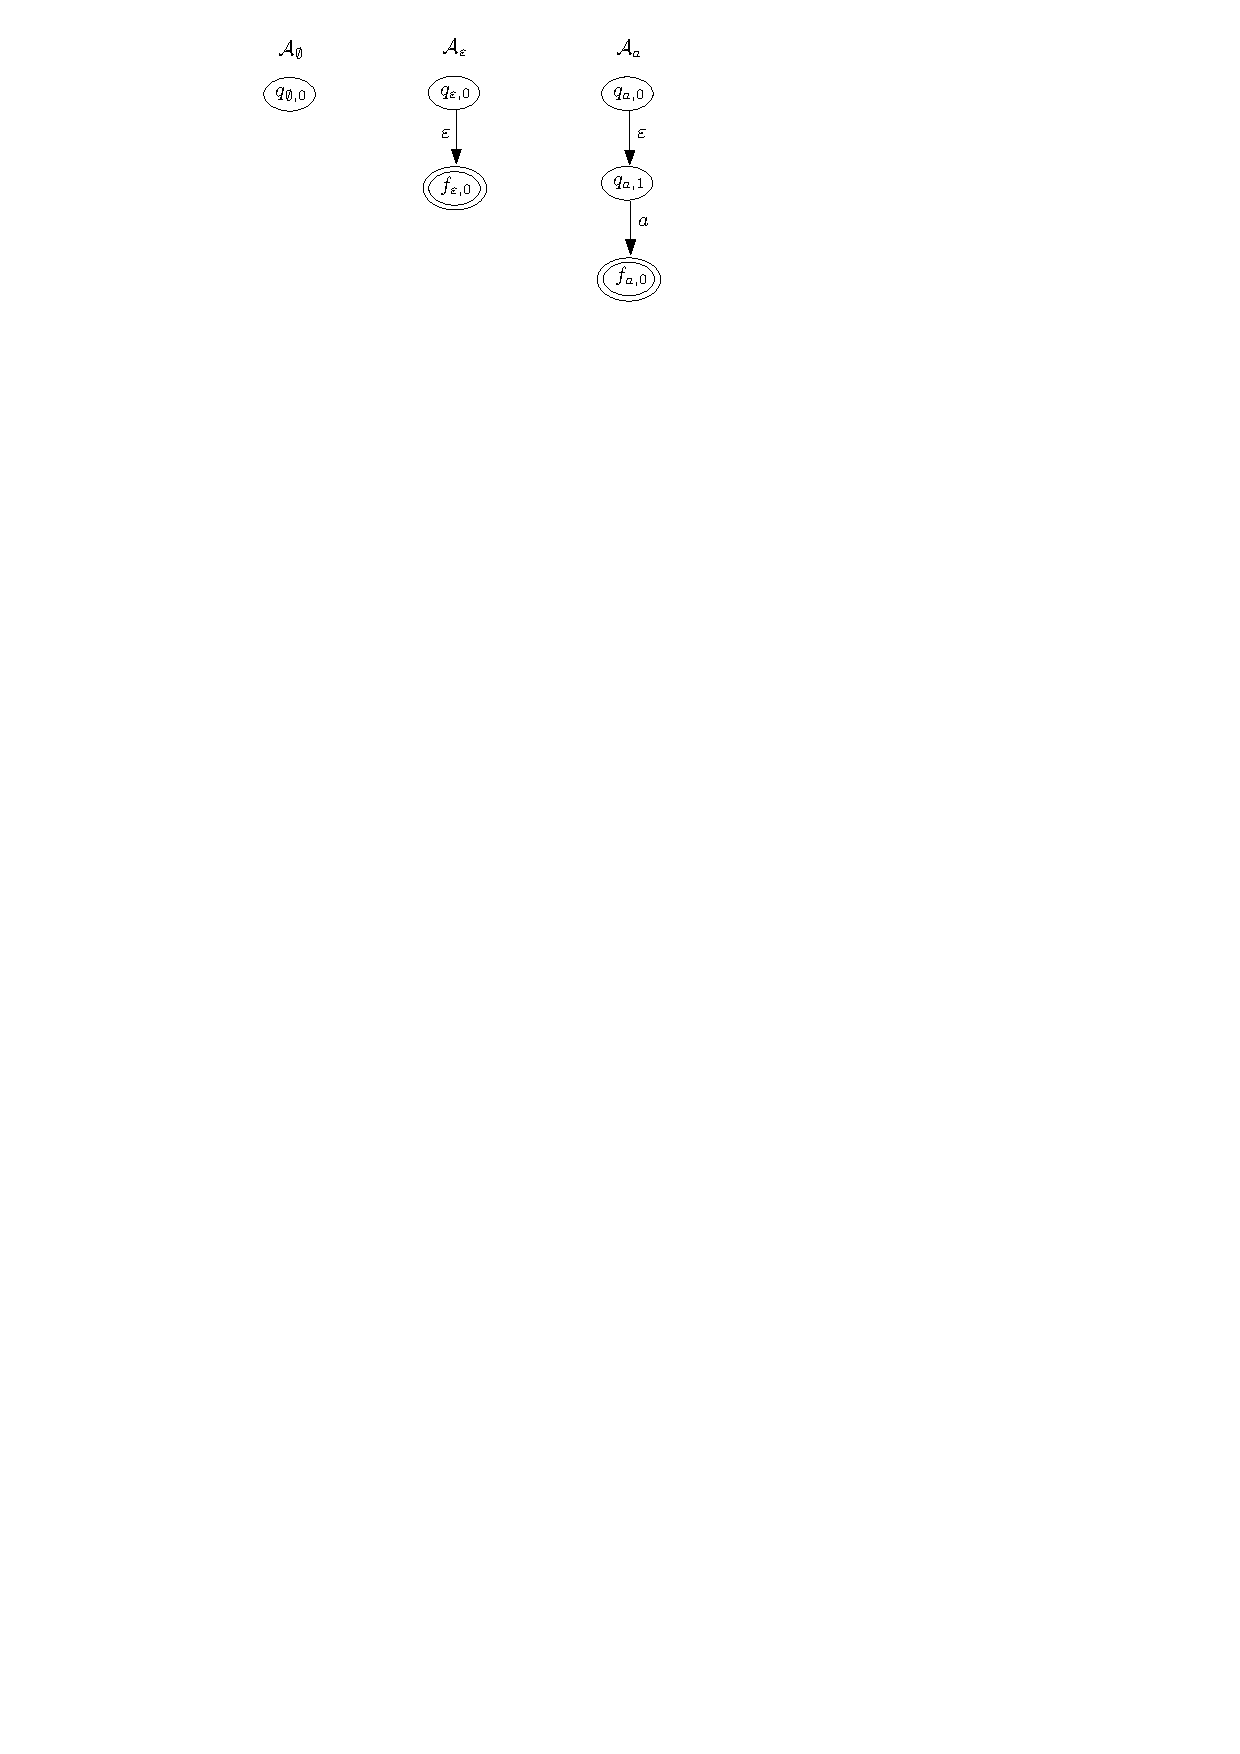
\includegraphics[width = 0.4\textwidth]{reg2pfa-0.pdf}
			\caption{The PFA $\cA_{\emptyset}$, $\cA_{\varepsilon}$, and $\cA_{a}$ }
			\label{fig-reg2pfa-0}
\end{figure}  
%%%%%%%%%%%%%%%%%%%%%%%%%%%%%%%%%%%%%%%%%%%%%%%%%%%%%%%%%%%%%%%%%%%%%%%%%%%%%%%%%%%%%%%%%%%%%%%%%%%%

		
\paragraph{Case $e = (e_1)$} $\cA_e = \cA_{e_1}$.
		

\paragraph{Case $e = [e_1 + e_2]$} Let 
\[\cA_{e_1} = (Q_{e_1}, \Sigma, \delta_{e_1}, \tau_{e_1}, q_{e_1,0}, (F_{e_1,1}, F_{e_1,2}))\] and 
\[\cA_{e_2} = (Q_{e_2}, \Sigma, \delta_{e_2}, \tau_{e_2}, q_{e_2,0}, (F_{e_2, 1}, F_{e_2,2}))\] 
then 
		%
\[\cA_e = (Q_{e_1} \cup Q_{e_2} \cup \{q_{e,0}\}, \Sigma,
		\delta_e, \tau_e, q_{e,0}, (F_{e_1,1} \cup F_{e_2,1}, F_{e_1,2} \cup F_{e_2,2}))\] where  
		\begin{itemize}
			\item $q_{e,0}  \not \in Q_{e_1} \cup Q_{e_2}$, 
			\item $\delta_e(q, a) = \delta_{e_i}(q, a)$ for every $i \in \{1,2\}$, $q \in Q_{e_i}$ and $a \in \Sigma$, 
			$\delta_e(q_{e,0}, a)  = ()$ for every $a \in \Sigma$, 
			%
			\item $\tau_e(q) = \tau_{e_i}(q)$ for every $q \in Q_{e_i}$ ($i =1,2$), $\tau_e(q_{e,0}) = ((q_{e_1,0},q_{e_2,0}); ())$.
		\end{itemize}
Fig.~\ref{fig-reg2pfa-1} depicts the construction.  	
		\begin{figure}[ht]
			\centering
			%\rule{\linewidth}{0cm}
			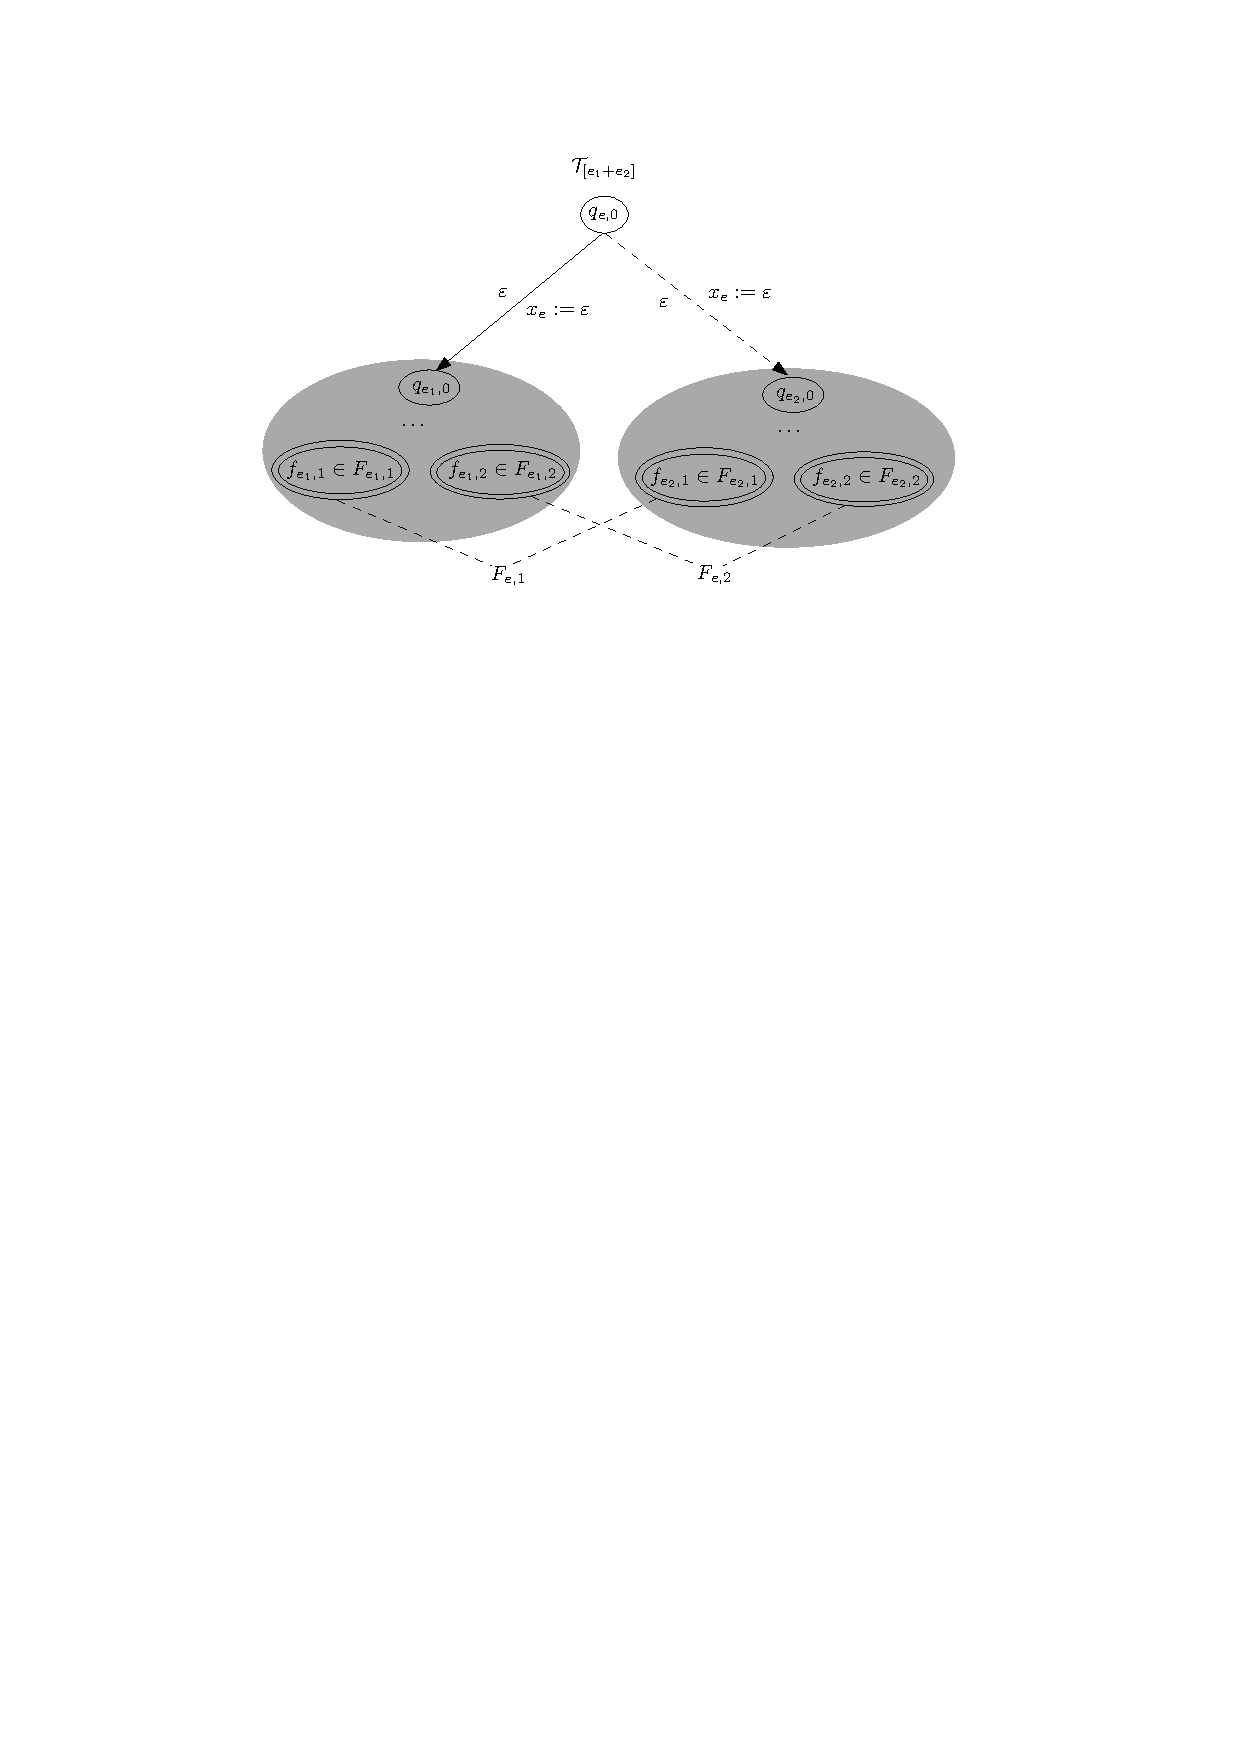
\includegraphics[width = 0.6\textwidth]{reg2pfa-1.pdf}
			\caption{The PFA $\cA_{[e_1+e_2]}$}
			\label{fig-reg2pfa-1}
		\end{figure}  

%%%%%%%%%%%%%%%%%%%%%%%%%%%%%%%%%%%%%%%%%%%%%%%%%%%%%%%%%%%%%%%%%%%%%%%%%%%%%%%%%%%%%%%%%%%%%%%%%%%%%

\paragraph{Case $e = [e_1^?]$} Let $\cA_{e_1} = (Q_{e_1}, \Sigma, \delta_{e_1}, \tau_{e_1}, q_{e_1,0}, (F_{e_1,1}, F_{e_1,2}))$, then 
\[\cA_e = (Q_{e_1} \cup \{q_{\varepsilon}\}, \Sigma,
		\delta_e, \tau_e, q_{e,0}, (\{q_{\varepsilon}\}, F_{e_1,2}))\]
where  
		\begin{itemize}
			\item $q_{e,0}  \not \in Q_{e_1}$
			\item $\delta_e(q, a) = \delta_{e_1}(q, a)$ for every $q \in Q_{e_1}$ and $a \in \Sigma$, $\delta_e(q_{e,0}, a)  = ()$ and $\delta_e(q_{\varepsilon}, a) = ()$ for every $a \in \Sigma$, 
			%
			\item $\tau_e(q) = \tau_{e_1}(q)$ for every $q \in Q_{e_1}$, $\tau_e(q_{e,0}) = ((q_{e_1,0},q_{\varepsilon}); ())$.
		\end{itemize}

Fig.~\ref{fig-reg2pfa-6} depicts the construction.
		\begin{figure}[ht]
			\centering
			%\rule{\linewidth}{0cm}
			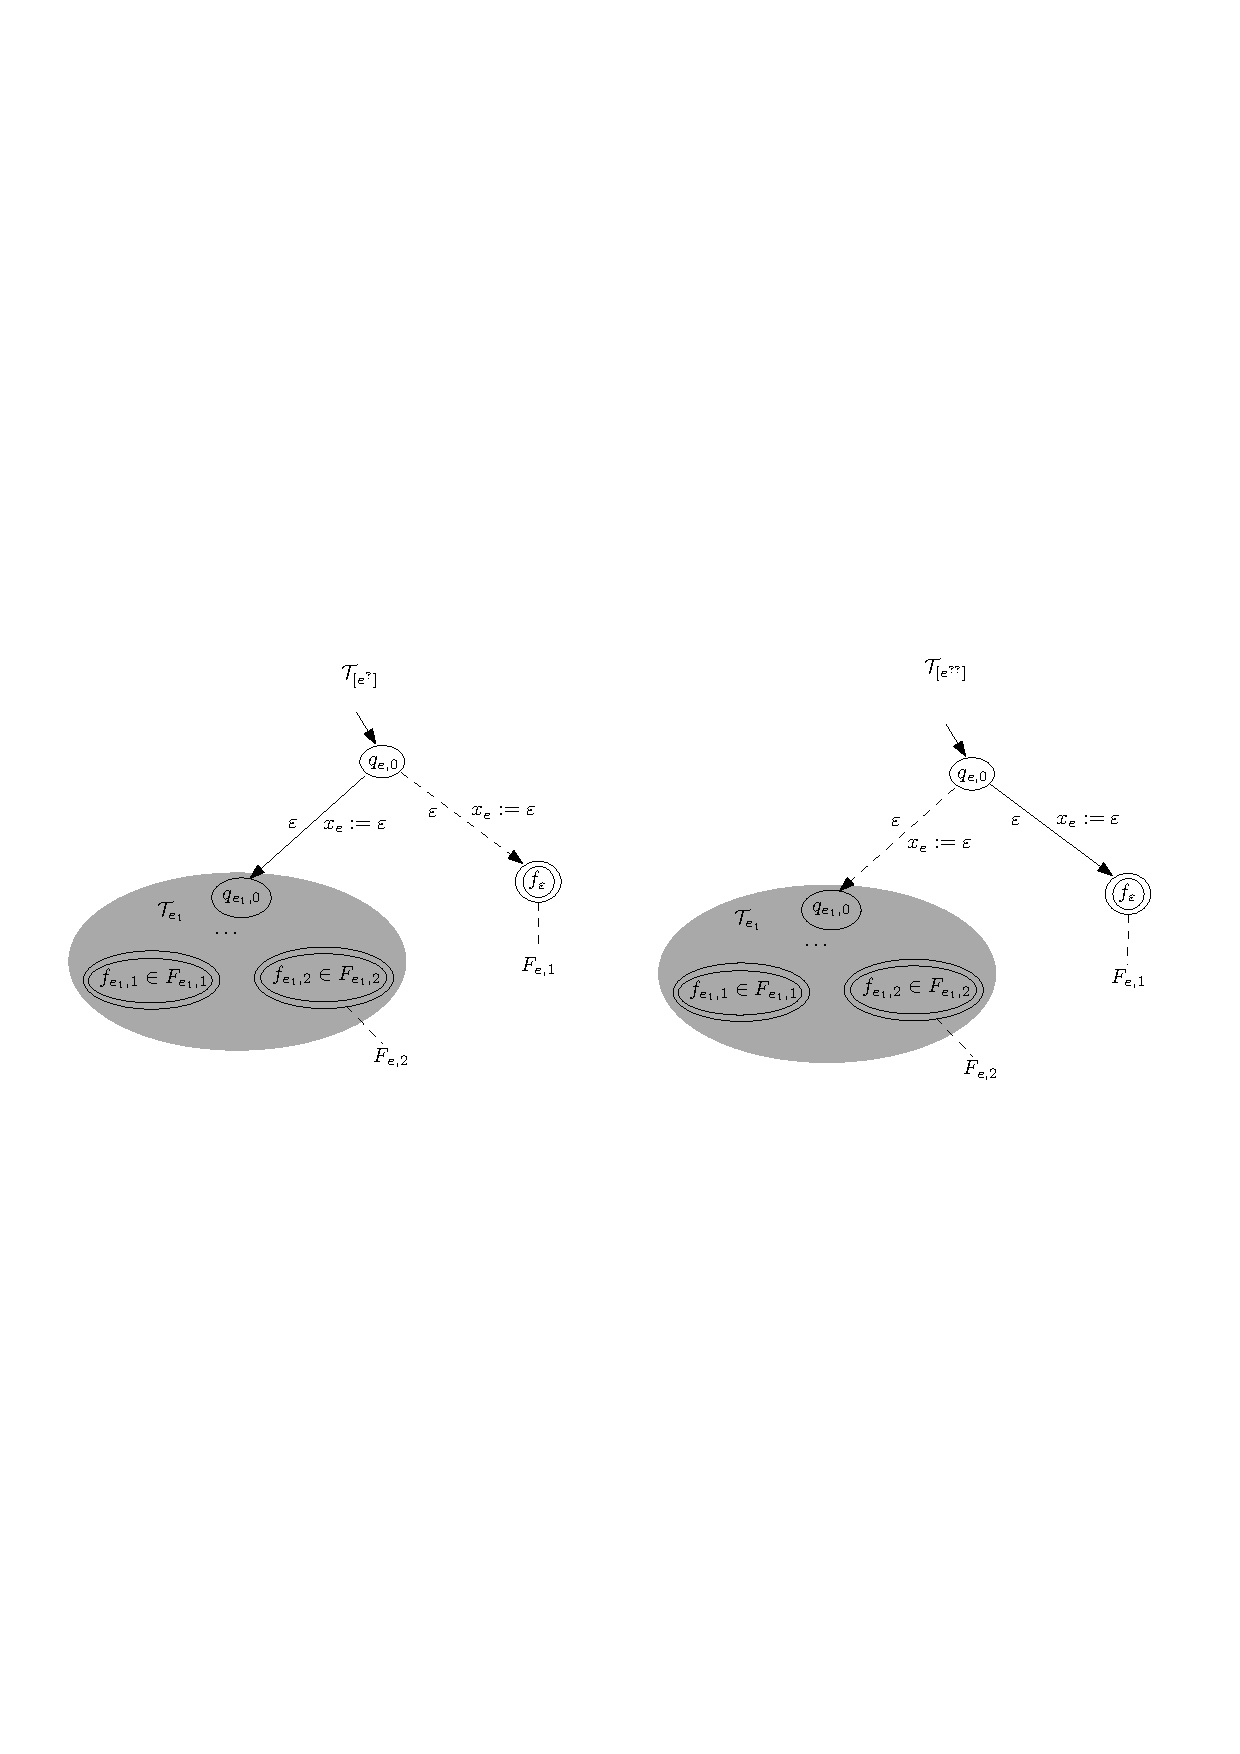
\includegraphics[width = 0.6\textwidth]{reg2pfa-6.pdf}
			\caption{The PFA $\cA_{[e_1^?]}$}
			\label{fig-reg2pfa-6}
		\end{figure}

%%%%%%%%%%%%%%%%%%%%%%%%%%%%%%%%%%%%%%%%%%%%%%%%%%%%%%%%%%%%%%%%%%%%%%%%%%%%%%%%%%%%%%%%%%%%%%%%%%%%%
\paragraph{Case $e = [e_1^{??}]$} 
Let $\cA_{e_1} = (Q_{e_1},
		\Sigma, \delta_{e_1}, \tau_{e_1}, q_{e_1,0}, (F_{e_1,1}, F_{e_1,2}))$. 
Then 
\[\cA_e = (Q_{e_1} \cup \{q_{\varepsilon}\}, \Sigma,
		\delta_e, \tau_e, q_{e,0}, (\{q_{\varepsilon}\}, F_{e_1,2}))\] 
where 
		\begin{itemize}
			\item $q_{e,0}  \not \in Q_{e_1}$
			\item $\delta_e(q, a) = \delta_{e_1}(q, a)$ for every $q \in Q_{e_1}$ and $a \in \Sigma$, $\delta_e(q_{e,0}, a)  = ()$ and $\delta_e(q_{\varepsilon}, a) = ()$ for every $a \in \Sigma$, 
			%
			\item $\tau_e(q) = \tau_{e_1}(q)$ for every $q \in Q_{e_1}$, $\tau_e(q_{e,0}) = ((q_{\varepsilon}, q_{e_1,0}); ())$.
		\end{itemize}
Fig.~\ref{fig-reg2pfa-7} depicts the construction. 
		\begin{figure}[ht]
			\centering
			%\rule{\linewidth}{0cm}
			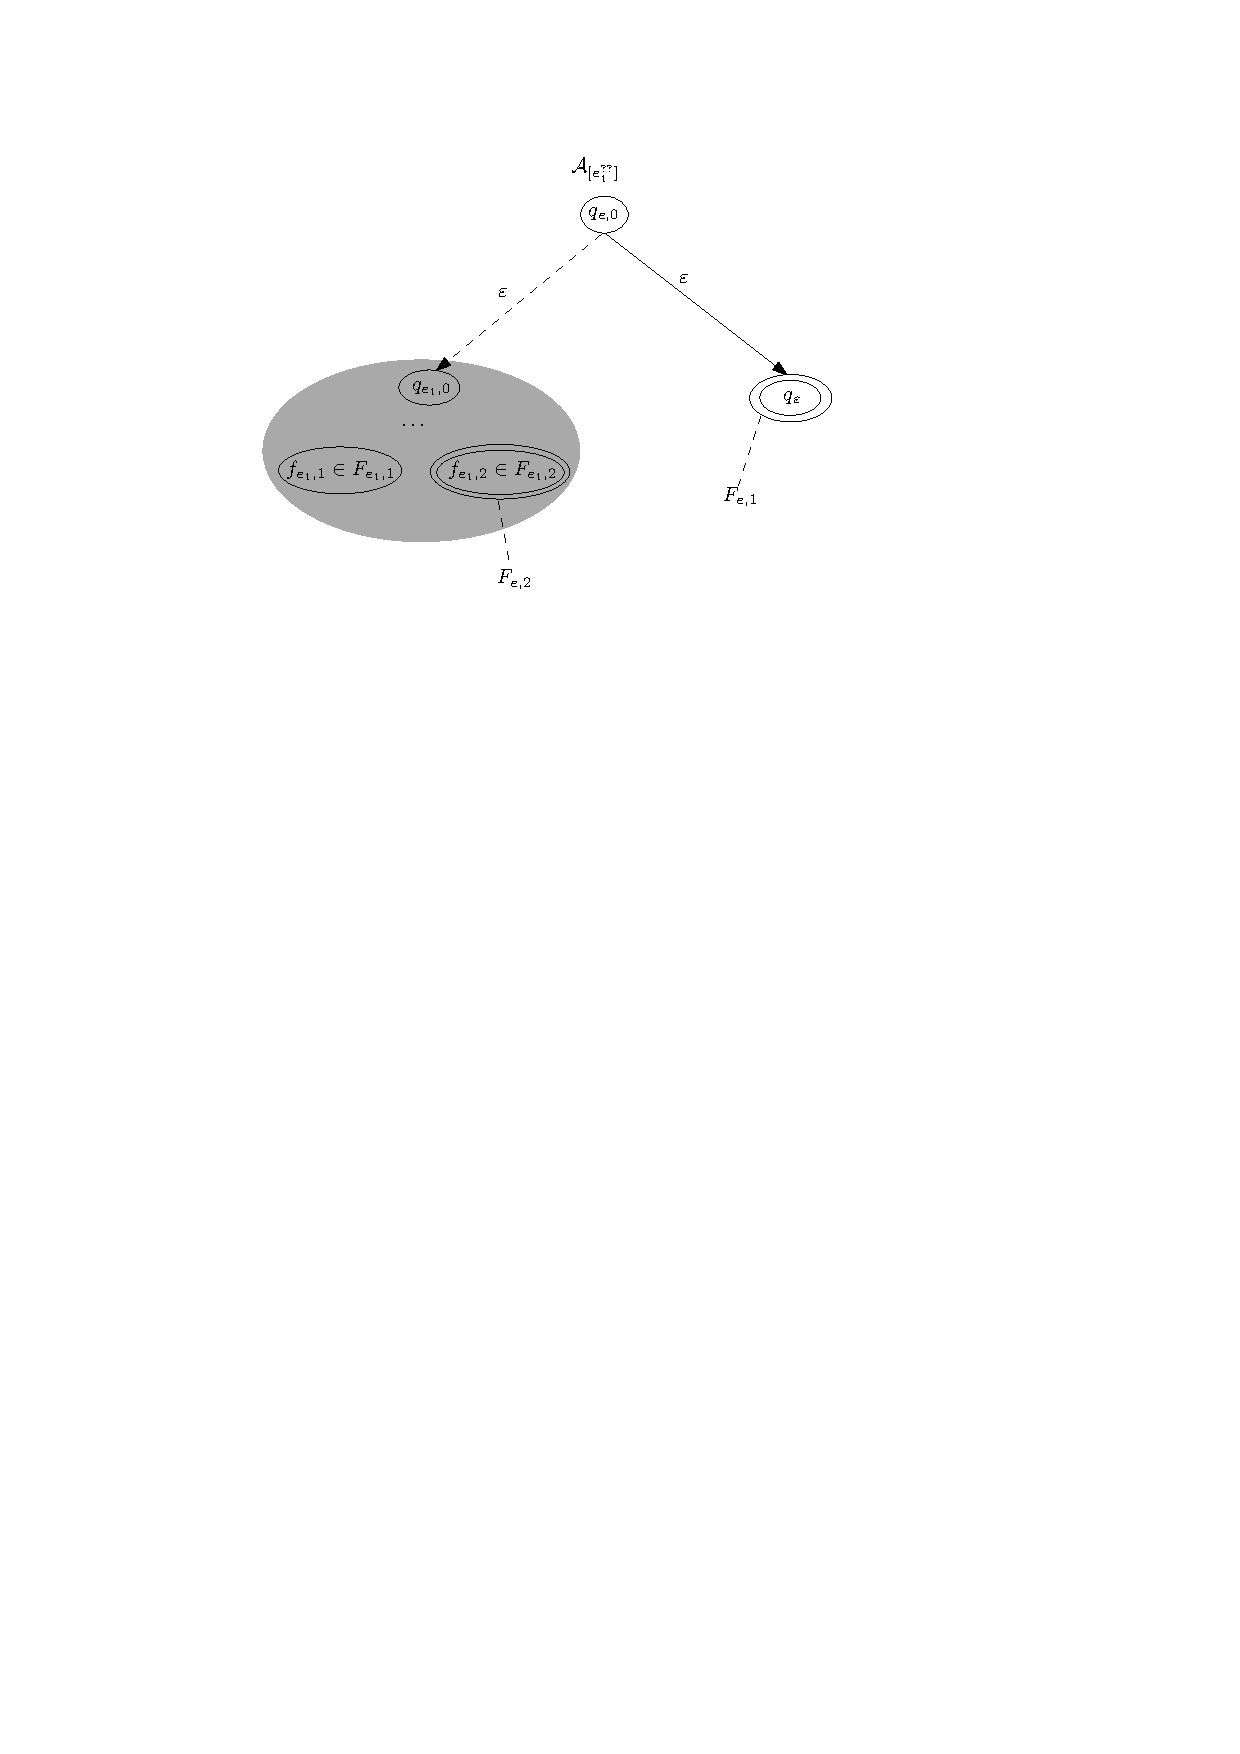
\includegraphics[width = 0.5\textwidth]{reg2pfa-7.pdf}
			\caption{The PFA $\cA_{[e_1^{??}]}$}
			\label{fig-reg2pfa-7}
		\end{figure}
	
%%%%%%%%%%%%%%%%%%%%%%%%%%%%%%%%%%%%%%%%%%%%%%%%%%%%%%%%%%%%%%%%%%%%%%%%%%%%%%%%%%%%%%%%%%%%%%%%%%%%%
\paragraph{Case $e = [e_1 \concat e_2]$} 
Let $\cA_{e_1} = (Q_{e_1}, \Sigma, \delta_{e_1}, \tau_{e_1}, q_{e_1,0}, (F_{e_1,1}, F_{e_1,2}))$, $\cA_{e_2} = (Q_{e_2}, \Sigma, \delta_{e_2}, \tau_{e_2}, q_{e_2,0}, (F_{e_2, 1}, F_{e_2,2}))$, and $\cA'_{e_2} = (Q'_{e_2}, \Sigma, \delta'_{e_2}, \tau'_{e_2}, q'_{e_2,0}, (F'_{e_2, 1}, F'_{e_2,2}))$ be a fresh copy of $\cA_{e_2}$, then 
		$\cA_e = ( Q_{e_1} \cup Q_{e_2} \cup Q'_{e_2}, \Sigma, \delta_e, \tau_e, q_{e_1,0},
		(F_{e_2,1}, F_{e_2,2} \cup F'_{e_2,1} \cup F'_{e_2,2}))$ where 
		\begin{itemize}
			\item for every $i \in \{1,2\}$, $q \in Q_{e_i}$ and $a \in \Sigma$, $\delta_e(q, a) = \delta_{e_i}(q, a)$,
			%
			\item for every $q' \in Q'_{e_2}$ and $a \in \Sigma$, $\delta_e(q', a) = \delta'_{e_2}(q',a)$, 
			%    
			\item for every $q \in Q_{e_2}$, $\tau_e(q) = \tau_{e_2}(q)$ and $\tau_e(q') = \tau'_{e_2}(q')$, 
			%
			\item for every $q \in Q_{e_1} \setminus (F_{e_1,1} \cup F_{e_1,2})$, $\tau_e(q) = \tau_{e_1}(q)$, for every $f_{e_1,1} \in F_{e_1,1}$, $\tau_e(f_{e_1,1}) = ((q_{e_2,0}); ())$, and for every $f_{e_1,2} \in F_{e_1,2}$, $\tau_e(f_{e_1,2}) = ((q'_{e_2,0}), ())$.
		\end{itemize}
 Fig.~\ref{fig-reg2pfa-2} depicts the construction. 
		\begin{figure}[ht]
			\centering
			%\rule{\linewidth}{0cm}
			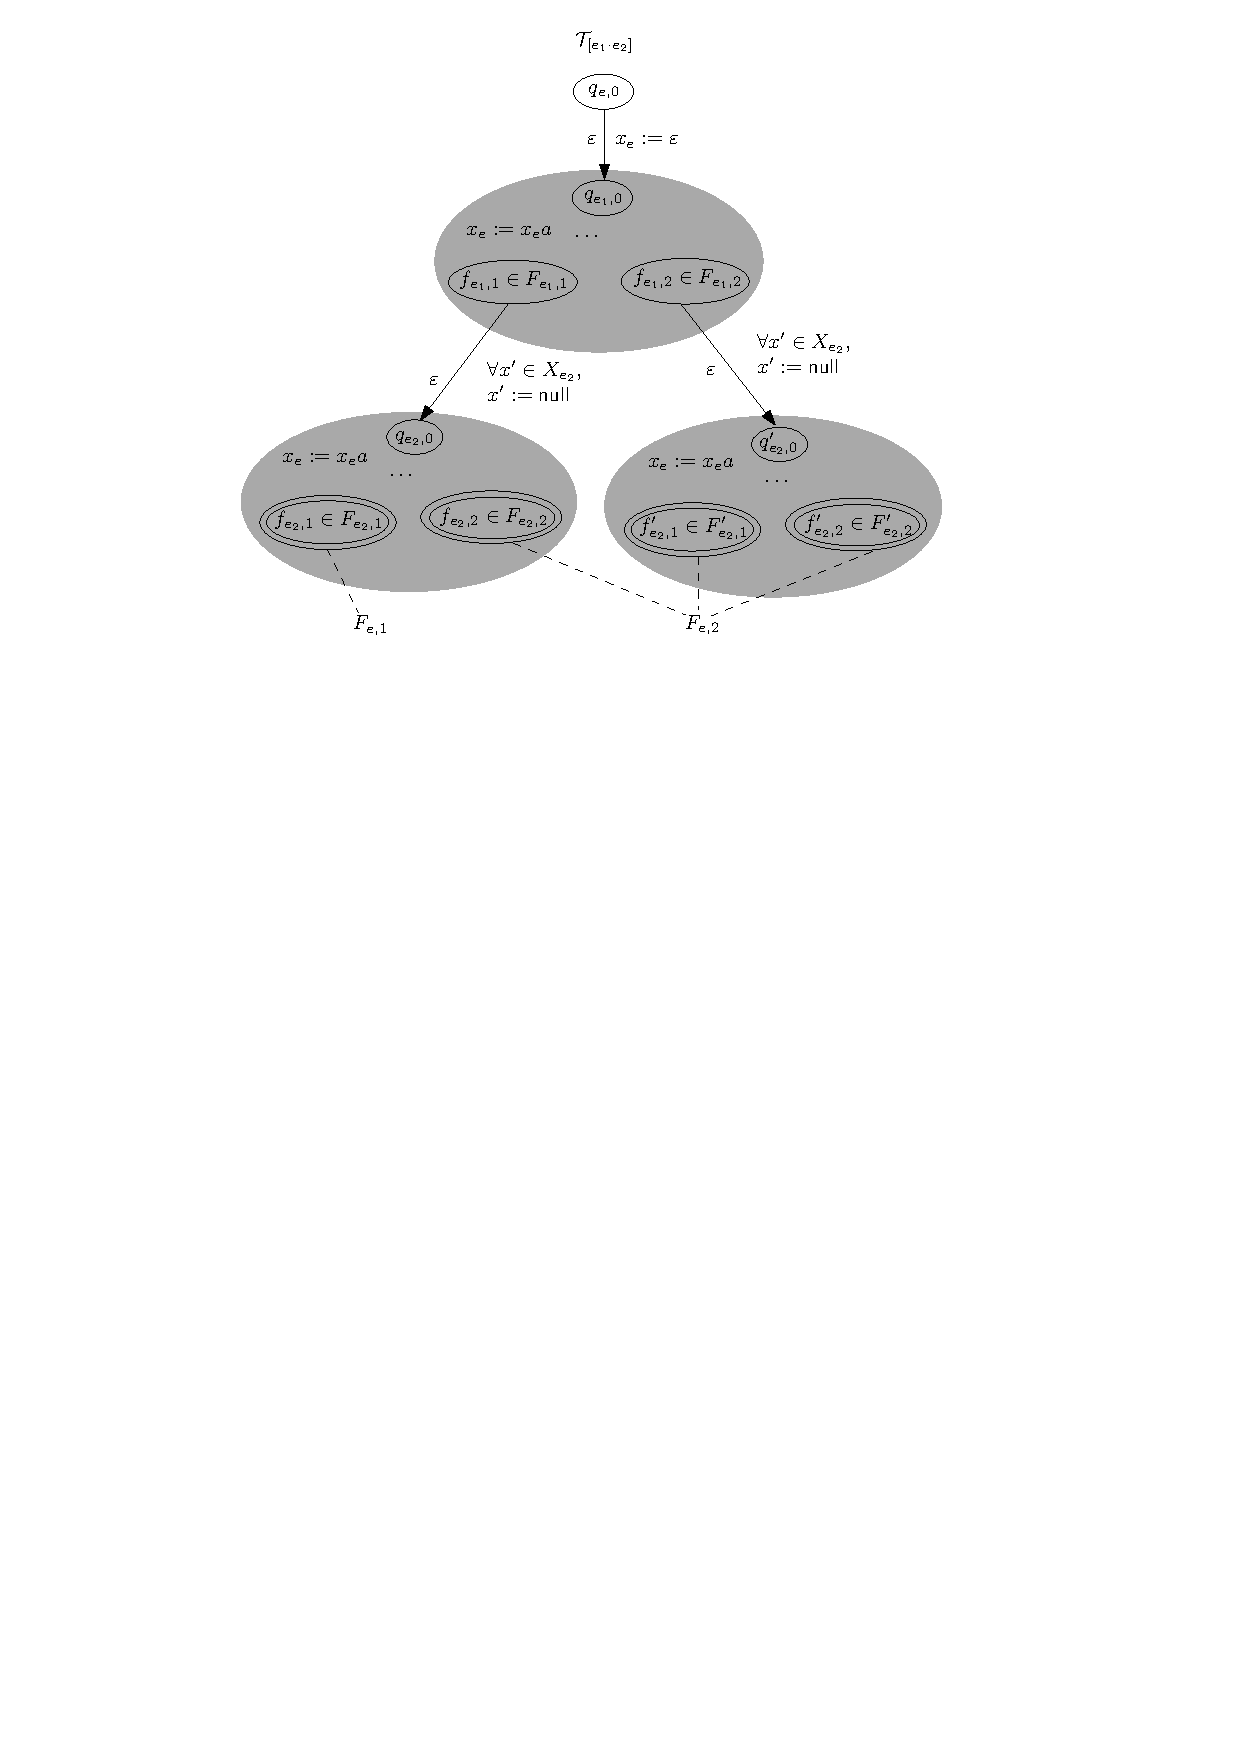
\includegraphics[width = 0.6\textwidth]{reg2pfa-2.pdf}
			\caption{The PFA $\cA_{[e_1\concat e_2]}$}
			\label{fig-reg2pfa-2}
		\end{figure}  
	

%%%%%%%%%%%%%%%%%%%%%%%%%%%%%%%%%%%%%%%%%%%%%%%%%%%%%%%%%%%%%%%%%%%%%%%%%%%%%%%%%%%%%%%%%%%%%%%%%%%%%

\paragraph{Case $e = [e_1^{\ast}]$} 
Let $\cA_{e_1} = (Q_{e_1}, \Sigma, \delta_{e_1}, \tau_{e_1}, q_{e_1,0}, (F_{e_1,1}, F_{e_1,2}))$. Then
\[ \cA_e = (Q_{e_1} \cup \{q_{e,0}, f_{e,0}, f_{e,1}\}, \Sigma, \delta_e, \tau_e, q_{e,0}, (\{f_{e,0}\}, \{f_{e,1}\}))\] where 
		\begin{itemize}
			\item $q_{e,0}, f_{e,0} \not \in Q_{e_1}$,
			
			\item for every $q \in Q_{e_1}$ and $a \in \Sigma$, $\delta_e(q, a) = \delta_{e_1}(q, a)$, 
			%moreover, $\delta(q_0, a) = \delta(f_0, a)  = ()$,
			
			\item for every $q \in Q_{e_1} \setminus (F_{e_1,1} \cup F_{e_1,2})$,  $\tau_e(q) = \tau_{e_1}(q)$, moreover, $\tau_e(q_{e,0}) = ((q_{e_1,0},f_{e,0}); ())$,  $\tau_e(q) = ((q_{e_1,0});())$ for every $q \in F_{e_1,1}$, $\tau_e(q) = ((q_{e_1,0}, f_{e,1});())$ for every $q \in F_{e_1,2}$, $\tau_e(f_{e,0}) =\tau_e(f_{e,1}) = (();())$. (Intuitively, the $\varepsilon$-transitions from $q_{e,0}$ to $q_{e_1,0}$ and $f_{e,0}$, from each $q \in F_{e_1,1}$ to $q_{e_1,0}$, and from $q \in F_{e_1,2}$ to $q_{e_1,0}$ and $f_{e,1}$ respectively are added, moreover, the $\varepsilon$-transition from $q_{e,0}$ to $f_{e,0}$ and from $q \in F_{e_1,2}$ to $f_{e,1}$ are of the lowest priority.)
		\end{itemize}

%%%%%%%%%%%%%%%%%%%%%%%%%%%%%%%%%%%%%%%%%%%%%%%%%%%%%%%%%%%%%%%%%%%%%%%%%%%%%%%%%%%%%%%%%%%%%%%%%%%%%
\paragraph{Case $e = [e_1^{+}]$} then $\cA_e$ is constructed as $\cA_{[e_1 \concat [e^\ast_1]]}$.
		
 
		

%%%%%%%%%%%%%%%%%%%%%%%%%%%%%%%%%%%%%%%%%%%%%%%%%%%%%%%%%%%%%%%%%%%%%%%%%%%%%%%%%%%%%%%%%%%%%%%%%%%%%
\paragraph{Case $e = [e_1^{\ast?}]$} Let  
		$\cA_{e_1} = (Q_{e_1}, \Sigma, \delta_{e_1}, \tau_{e_1}, q_{e_1,0}, (F_{e_1,1}, F_{e_1,2}))$. Then 
\[\cA_e = (Q_{e_1} \cup \{q_{e,0}, f_{e,0}, f_{e,1}\}, \Sigma, \delta_e, \tau_e, q_{e,0}, (\{f_{e,0}\}, \{f_{e,1}\}))\]  where 
		\begin{itemize}
			\item $q_{e,0}, f_{e,0} \not \in Q_{e_1}$,
			
			\item for every $q \in Q_{e_1}$ and $a \in \Sigma$, $\delta_e(q, a) = \delta_{e_1}(q, a)$, 
			%moreover, $\delta(q_0, a) = \delta(f_0, a)  = ()$,
			
			\item for every $q \in Q_{e_1} \setminus (F_{e_1,1} \cup F_{e_1,2})$,  $\tau_e(q) = \tau_{e_1}(q)$, moreover, $\tau_e(q_{e,0}) = ((f_{e,0}, q_{e_1,0}); ())$,  $\tau_e(q) = ((q_{e_1,0});())$ for every $q \in F_{e_1,1}$, $\tau_e(q) = ((f_{e,1}, q_{e_1,0});())$ for every $q \in F_{e_1,2}$, $\tau_e(f_{e,0}) =\tau_e(f_{e,1}) = (();())$. (Intuitively, the $\varepsilon$-transitions from $q_{e,0}$ to $f_{e,0}$ and $q_{e_1,0}$ , from each $q \in F_{e_1,1}$ to  $q_{e_1,0}$, and from each $q \in F_{e_1,2}$ to $f_{e,1}$ and $q_{e_1,0}$ respectively are added, moreover, the $\varepsilon$-transition from $q_{e,0}$ to $q_{e_1,0}$ and from $q \in F_{e_1,2}$ to $q_{e_1,0}$ are of the lowest priority.)
		\end{itemize}

 
%%%%%%%%%%%%%%%%%%%%%%%%%%%%%%%%%%%%%%%%%%%%%%%%%%%%%%%%%%%%%%%%%%%%%%%%%%%%%%%%%%%%%%%%%%%%%%%%%%%%%
\paragraph{Case $e = [e_1^{+?}]$} then $\cA_e$ is constructed as $\cA_{[e_1 \concat [e_1^{*?}]]}$.

Fig.~\ref{fig-reg2pfa-3} depicts the construction. 
\begin{figure}[ht]
	\centering
	%\rule{\linewidth}{0cm}
	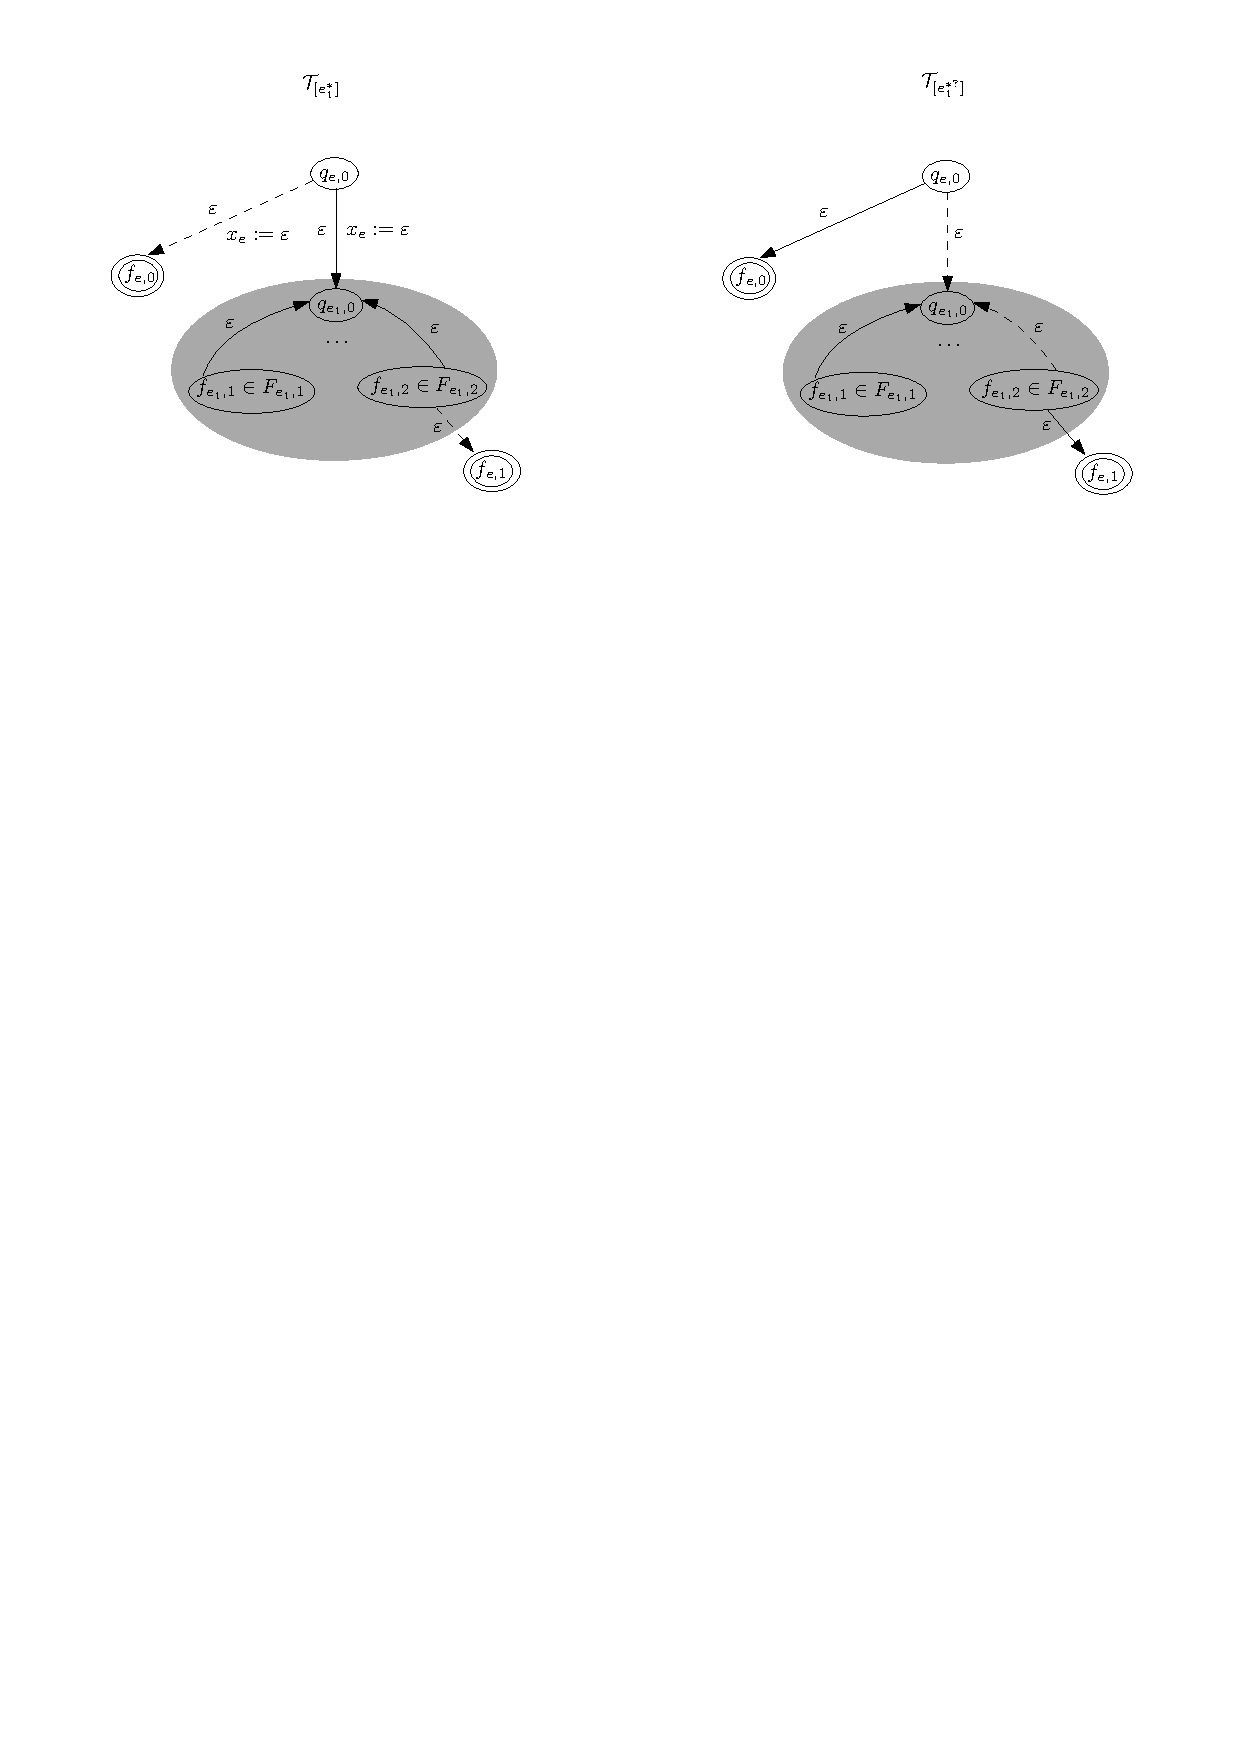
\includegraphics[width = 0.8\textwidth]{reg2pfa-3.pdf}
	\caption{The PFA $\cA_{[e_1^\ast]}$ and $\cA_{[e_1^{\ast?}]}$}
	\label{fig-reg2pfa-3}
\end{figure}

%%%%%%%%%%%%%%%%%%%%%%%%%%%%%%%%%%%%%%%%%%%%%%%%%%%%%%%%%%%%%%%%%%%%%%%%%%%%%%%%%%%%%%%%%%%%%%%%%%%%%
\paragraph{Case $e = [e_1^{\{m_1,m_2\}}]$} Then $\cA_e$ is constructed as the concatenation of $\cA_{e_1^{m_1}}$ and $\cA^\prime_{e_1^{\{1,m_2-m_1\}}}$, where $\cA_{e_1^{m_1}}$ is the PFA corresponding to consecutive concatenations of $m_1$ copies of $e_1$, and $\cA^\prime_{e_1^{\{1,m_2-m_1\}}}$ is illustrated in Fig.~\ref{fig-reg2pfa-4}, which consists of $m_2-m_1$ copies of $\cA_{e_1}$, say $(\cA^{(i)}_{e_1})_{i \in [m_2-m_1]}$, as well as the $\varepsilon$-transition from $q^{(1)}_{e_1,0}$ to a fresh state $f^\prime_0$ (of the lowest priority), and the $\varepsilon$-transitions from each $f^{(i)}_{e_1,2} \in F^{(i)}_{e_1,2}$ to $q^{(i+1)}_{e_1,0}$ (of the highest priority), and a fresh state $f^\prime_1$ (of the lowest priority). The accepting states of $\cA^\prime_{e_1^{\{1,m_2-m_1\}}}$ are $(\{f_0'\},\{f_1'\})$. (Intuitively, each $\cA^{(i)}_{e_1}$ accepts only nonempty strings, thus $f^{(i)}_{e_1,1} \in F^{(i)}_{e_1,1}$ contains no outgoing transitions in $\cA^\prime_{e_1^{\{1,m_2-m_1\}}}$. )
		%
		\begin{figure}[ht]
			\centering
			%\rule{\linewidth}{0cm}
			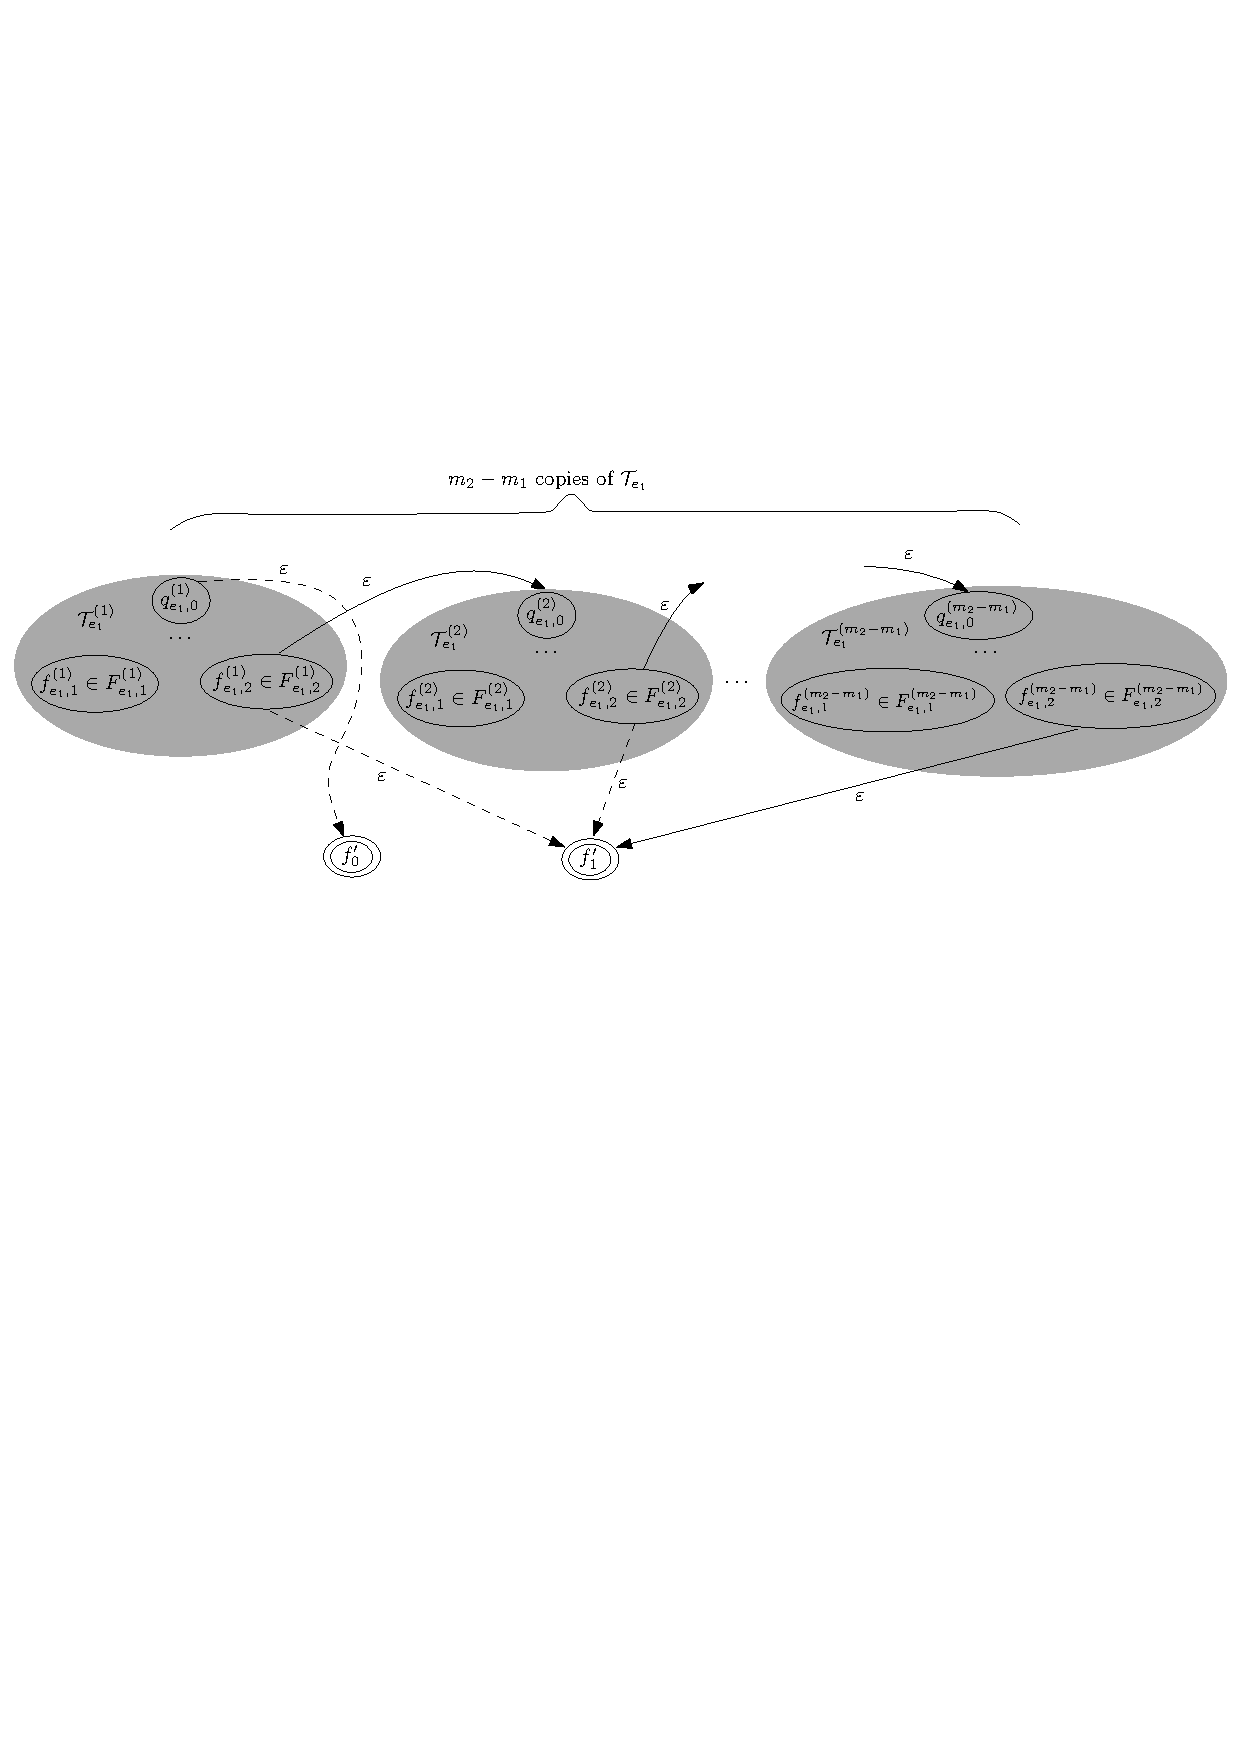
\includegraphics[width = 0.8\textwidth]{reg2pfa-4.pdf}
			\caption{The PFA $\cA^\prime_{e_1^{\{1,m_2-m_1\}}}$}
			\label{fig-reg2pfa-4}
		\end{figure}  


%%%%%%%%%%%%%%%%%%%%%%%%%%%%%%%%%%%%%%%%%%%%%%%%%%%%%%%%%%%%%%%%%%%%%%%%%%%%%%%%%%%%%%%%%%%%%%%%%%%%%
\paragraph{Case $e = [e_1^{\{m_1,m_2\}?}]$} Then $\cA_e$ is constructed as the concatenation of $\cA_{e_1^{m_1}}$ and $\cA^\prime_{e_1^{\{1,m_2-m_1\}?}}$, where $\cA^\prime_{e_1^{\{1,m_2-m_1\}?}}$ is illustrated in Fig.~\ref{fig-reg2pfa-5}, which is the same as $\cA^\prime_{e_1^{\{1,m_2-m_1\}}}$ in Fig.~\ref{fig-reg2pfa-4}, except that the priorities of $\varepsilon$-transition from $q^{(1)}_{e_1,0}$ to $f^\prime_0$ has the highest priority and  the priorities of $\varepsilon$-transitions from each $f^{(i)}_{e_1,2} \in F^{(i)}_{e_1,2}$ to $f^\prime_1$ are reversed.
		\begin{figure}[ht]
			\centering
			%\rule{\linewidth}{0cm}
			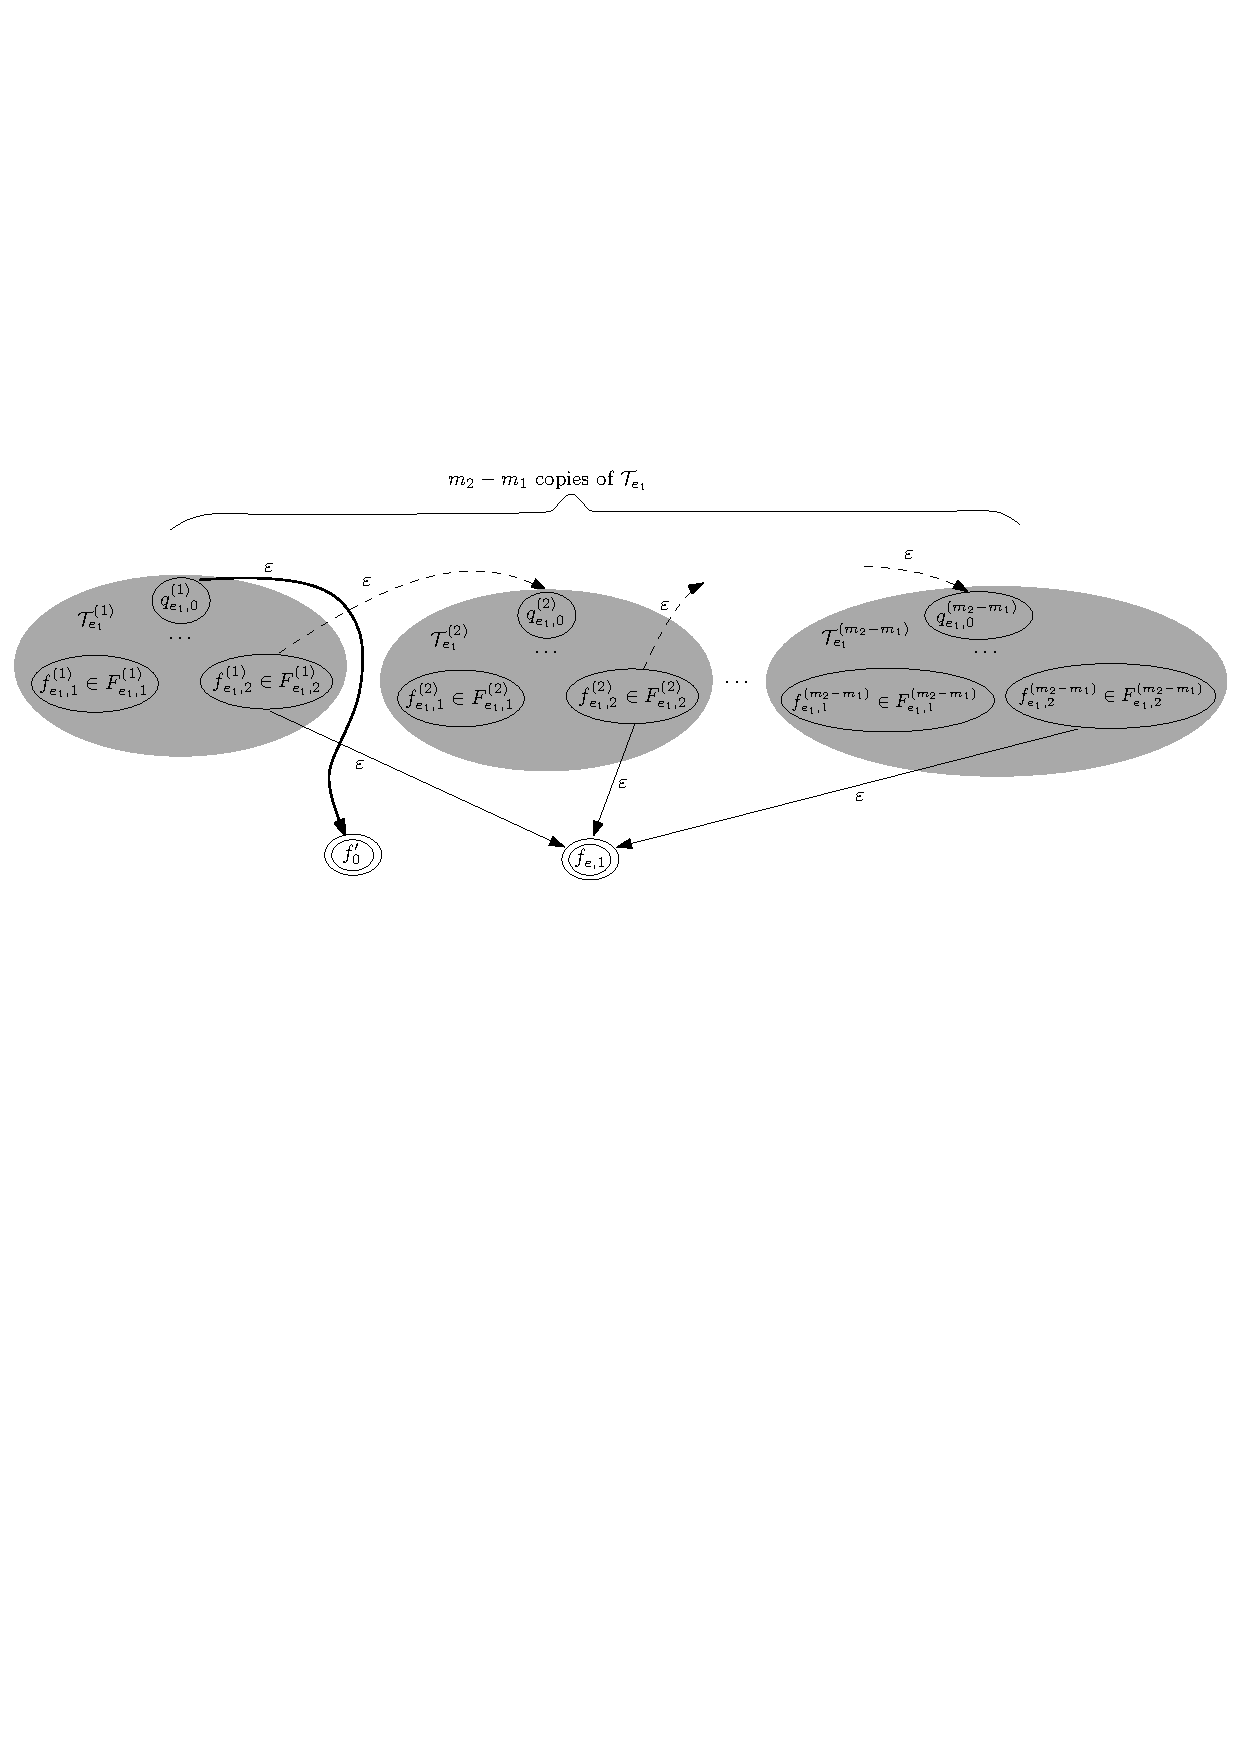
\includegraphics[width = 0.8\textwidth]{reg2pfa-5.pdf}
			\caption{The PFA $\cA^\prime_{e_1^{\{1,m_2-m_1\}?}}$}
			\label{fig-reg2pfa-5}
		\end{figure}  
%%%%%%%%%%%%%%%%%%%%%%%%%%%%%%%%%%%%%%%%%%%%%%%%%%%%%%%%%%%%%%%%%%%%%%%%%%%%%%%%%%%%%%%%%%%%%%%%%%%%%%%%

 %can be constructed 
%(in linear time)

% such that 
%	\begin{itemize}
%		\item $\cA_e$ has a unique initial state without incoming transitions and a unique final state without outgoing transitions,
%		%
%		\item for subexpression $e'$ of $e$, $\cA_e$ contains at least one isomorphic copy of $\cA_{e'}$ (i.e. the PFA constructed for $e'$), denoted by ${\sf Sub}_{e'}[\cA_e]$. 
%	\end{itemize}

%Let us use ${\sf Sub}_{e'}[\cA_e]$ to denote the isomorphic copy of $\cA_{e'}$ in $\cA_e$, as mentioned in Proposition~\ref{prop-rwre-to-pfa}.

%\begin{proof}
%	For any $e \in \cgexp$, a PFA $\cA_e$ is constructed recursively in the sequel. The constructed PFA $\cA_e$ satisfies that 
%	\begin{itemize}
%		\item it has a unique initial state without incoming transitions and each of its final states has no outgoing transitions,
%		\item all the transitions out of the initial state are $\varepsilon$-transitions, 
%		\item the set of final states is divided into two disjoint subsets $F_1, F_2$ such that for each $w \in \Sigma^*$ satisfying that $q_0 \xrightarrow[\cA_e]{w} q$ for some $q \in F_1$ (resp. $q \in F_2$), $w = \varepsilon$ (resp. $w \neq \varepsilon$).
%	\end{itemize}


